\documentclass{article}
\usepackage
[
        a4paper,% other options: a3paper, a5paper, etc
        left=2.5cm,
        right=2.5cm,
        top=2.5cm,
        bottom=3.5cm,
        % use vmargin=2cm to make vertical margins equal to 2cm.
        % use hmargin=3cm to make horizontal margins equal to 3cm.
        % use margin=3cm to make all margins  equal to 3cm.
]
{geometry}
%\usepackage[utf8]{inputenc}
%\usepackage{amssymb}
%\usepackage{graphicx}
\usepackage{hyperref}
%\usepackage[demo]{graphicx}
\usepackage{graphicx}
\usepackage{subcaption}
\usepackage[ruled,linesnumbered]{algorithm2e}
\usepackage{amsmath}
\usepackage{lscape}



\title{Galaxy formation and evolution in the IGIMF theory}
\author{Sarah Yousefizadeh$^{1}$ \\
$^{1}$ yousefi@iasbs.ac.ir
} 
\date{\today}

\begin{document}
\maketitle
%\begin{abstract}
%abs goes here 
 
% \end{abstract}
% \pagebreak

%\begin{document}
 
\flushbottom % Makes all text pages the same height

\maketitle % Print the title and abstract box
\tableofcontents % Print the contents section

\thispagestyle{empty} % Removes page numbering from the first page

%----------------------------------------------------------------------------------------
%	ARTICLE CONTENTS
%----------------------------------------------------------------------------------------

\section*{Introduction}
\addcontentsline{toc}{section}{Introduction} % Adds this section to the table of contents
The initial distribution of stellar masses as the outcome of star formation is a fundamentally important key for understanding the evolution of stellar systems on star-cluster and
galaxy scales. \cite{yan-kroupa}. 
\\The stellar initial mass function $(IMF, \xi(m))$ describes the distribution of masses of stars, whereby $dN = \xi(m)dm$ is the number of stars formed in the mass interval $m, m + dm$. It is one of the most important distribution functions in astrophysics as stellar evolution is generally determined by the mass of the stars. The IMF therefore regulates the chemical enrichment history of galaxies, as well as their mass-to-light ratios and influences their dynamical evolution.\cite{kroupa-weidner} \\
Theoretically unexpected, the IMF is found to be invariant through a large range of conditions like gas densities and metallicites (Kroupa 2001, 2002;
Chabrier 2003; Elmegreen et al. 2008; Bastian et al. 2010; Kroupa et al. 2013) and is well described by the canonical IMF (Appendix B).\\ Though, it has to be kept in mind that often the concept of an universal IMF is understood as a constant slope
of the IMF, ignoring the upper and lower mass limits. As the slope (for stellar masses above $1 M_{\odot}$ ) has been found to be
constant (within the uncertainties) for star clusters in the Milky Way and the Magellanic clouds (Kroupa 2002; Massey 2003),
an invariant IMF is widely used to not only describe individual star clusters but also stellar populations of whole galaxies.\\ But,
the question remains whether the IMF, derived from and tested on star cluster scales, is the appropriate stellar distribution
function for complex stellar populations like galaxies. \\ In this context, it has emerged that if all the stars in a galaxy form
with a canonical IMF 1 and all these IMFs of all star-forming events (spatially and temporally correlated star formation
events/CSFE) are added up the resulting integrated galactic initial mass function of stars (IGIMF) differs substantially from the canonical IMF. It should be pointed out here that the principal concept of the IGIMF - the galaxy-wide IMF (= IGIMF)
of a galaxy is always the sum of all star-formation events within a galaxy - is in any case always true.
\\
The ingredients for the IGIMF as applied here are listed as follows:
\begin{itemize}
	\item The IMF, $\xi(m)$, within star clusters is assumed to be canonical (see Appendix B),
	\item the CSFEs populate an embedded-cluster mass function (ECMF), which is assumed to be a power-law of the form,\\
		$\xi_{ecl}(M_{ecl}) = dN/dM_{ecl} \propto M_{ecl}^{-\beta}$
	\item the relation between the most-massive star in a cluster, $m_{max}$ , and the stellar mass of the embedded cluster, $M_{ecl}$
	(Weidner Kroupa 2004, 2006; Weidner et al. 2010),
	\item the relation between the star-formation rate (SFR) of a galaxy and the most-massive young (< 10 Myr) star cluster,
	$log_{10} (M_{ecl,max} ) = 0.746 \times log_{10}(SF R) + 4.93$ (Weidner et al. 2004).
	
\end{itemize}

\section{The universal IMF}

The available constraints can be conveniently summarized by the	multiple-part power-law IMF (see Kroupa 2001b for details),\\ \\ $\xi(m) \propto  m^{-\alpha_{i}}$\\ \\
where,\\ \\
$\alpha_{0}= +0.3\pm0.7,    0.01\leq \frac{m}{M_{\odot}} \le0.08,$\\
$\alpha_{1}= +1.3\pm0.5,     0.08\leq \frac{m}{M_{\odot}} \le 0.50,$\\
$\alpha_{2}= +2.3\pm0.3,     0.5\leq \frac{m}{M_{\odot}} \le 1.00,$\\
$\alpha_{3}= +2.3\pm0.7,     1.00\leq \frac{m}{M_{\odot}} ,$\\ \\ and $\xi(m)dm$ is the number of single stars in the mass interval $m$ to
	$m+dm$ The uncertainties correspond approximately to 99 percent confidence intervals for $m \geq 0.5 M_{\odot}$, and to a 95 percent confidence interval for $1-0.5 M_{\odot}$. Below $0.08 M_{\odot}$
	the confidence range is not well determined.

\section{THE $m_{max}-M_{ecl}$ RELATION}
The $m_{max}-M_{ecl}$ relation, as shown in Fig.\ref{fig:max-mecl}has been analytically presented in Weidner  Kroupa (2004), observationally
established by Weidner  Kroupa (2006) and refined in Weidner et al. (2010), while already briefly theoretically discussed
in Reddish (1978).\\
It signifies that the typical upper mass limit to which the IMF is sampled, m max , changes systematically
with the stellar mass of the cluster, $M_{ecl}$ .
\begin{figure}[h]\centering
	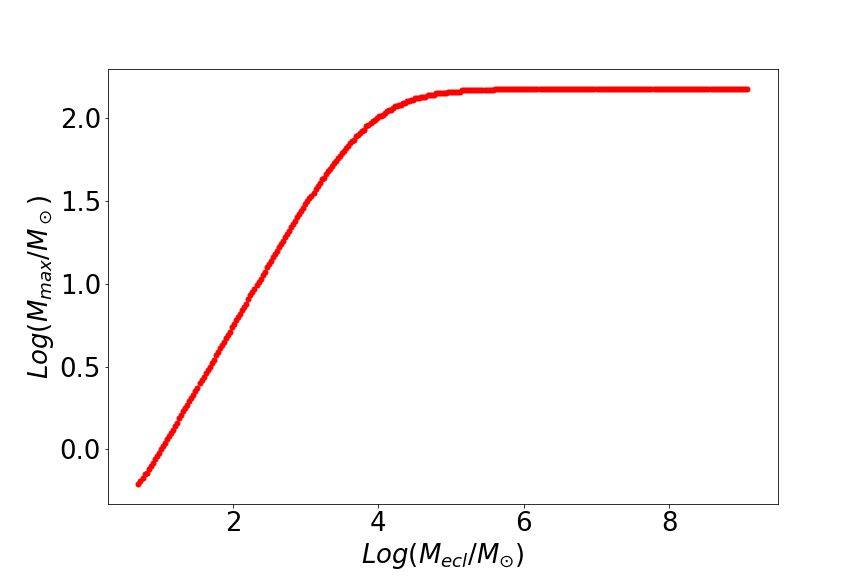
\includegraphics[width=0.7\linewidth]{max-melc.png}
	\caption{The mass of the most-massive star $(m_{max})$ in an embedded cluster versus the stellar mass of the young dynamically
		un-evolved ”embedded” cluster $(M_{ecl})$.The solid lines through the data points are the analytical $m_{max}-M_{ecl}$
		relation when using a fundamental upper mass limit, $m_{max,*}$ , of $150 M_{\odot}$.}
	\label{fig:max-mecl}
\end{figure}
For the clusters for which the number of stars above a mass limit or within a mass range are given in the literature,
the cluster mass,  $M_{ecl}$  , is calculated by assuming a canonical IMF from $0.01$ to $150 M_{\odot}$ and extrapolating
to the total population from the observational mass limits.
\subsection{The maximum stellar mass and cluster formation}
Assuming the stellar IMF is a continuous density distribution function and that
clusters are filled with stars distributed according to the stellar IMF, this can
be generalized by stating that each cluster can have only one most massive star,
\begin{equation}
1=\int_{m_{max}}^{m_{max*}}\xi(m')dm',
\end{equation}
with,
\begin{equation}
M_{}ecl}(m_{max})=\int_{m_{low}}^{m_{max}} m' \xi(m')dm',
\end{equation}
as a further condition, as above. These two equations need to be solved numeri-
cally and give the semi-analytical relation $ m_{max}= \eta (M_{ecl} )$(Weidner & Kroupa
2004). It is plotted in fig.\ref{fig:max-mecl}.
A compilation of clusters from the literature for which the cluster mass and
the initial mass of the heaviest star can be estimated (Weidner & Kroupa 2006)
shows that the cluster mass indeed appears to have a limiting influence on the
stellar mass within it. The observational data are plotted in Fig. \ref{fig:ko-re}, finding
rather excellent agreement with the semi-analytical description above.
\begin{figure}[h]\centering
	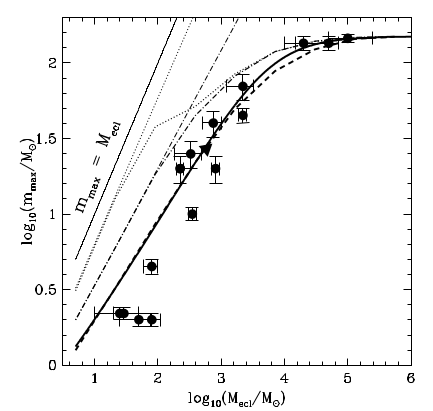
\includegraphics[width=0.7\linewidth]{ko-rev.png}
	\caption{The thick solid line shows the dependence of the mass of the most-
		massive star in a cluster on the cluster mass according to the semi-analytical	model. The thick dashed line shows the mean maximum stellar mass for sorted
		sampling. The dot-dashed lines are mass-constrained random-sampling results	with a physical upper mass limit of $m_{max*}=150M_{\odot}$ (thick line) and $10^6 M_{\odot}$(thin line). Pure random sampling models are plotted as dotted lines. The
		thick one is sampled to $m_{max*}=150M_{\odot}$ while the thin one up to $10^6 M_{\odot}$.
		The thin solid line shows the identity relation, where a “cluster” consists only of one star. The dots with error bars are observed clusters, while the triangle is a result from a star-formation simulation with an SPH code (Bonnell et al.2003). Taken from Weidner & Kroupa (2006).}
	\label{fig:ko-re}
\end{figure}



\section{The maximum stellar mass and cluster formation}
Assuming the stellar IMF is a continuous density distribution function and that
clusters are filled with stars distributed according to the stellar IMF, this can
be generalized by stating that each cluster can have only one most massive star,
\begin{equation}
1=\int_{m_{max}}^{m_{max*}}\xi(m')dm',
\end{equation}
with,
\begin{equation}
M_{ecl}(m_{max})=\int_{m_{low}}^{m_{max}} m' \xi(m')dm',
\end{equation}
as a further condition, as above. These two equations need to be solved numerically and give the semi-analytical relation $ m_{max}= \eta (M_{ecl} )$(Weidner & Kroupa
2004). It is plotted in figure \ref{fig:max-mecl}.
\begin{figure}
	\centering
	\begin{subfigure}[b]{0.4\textwidth}
%		\centering
		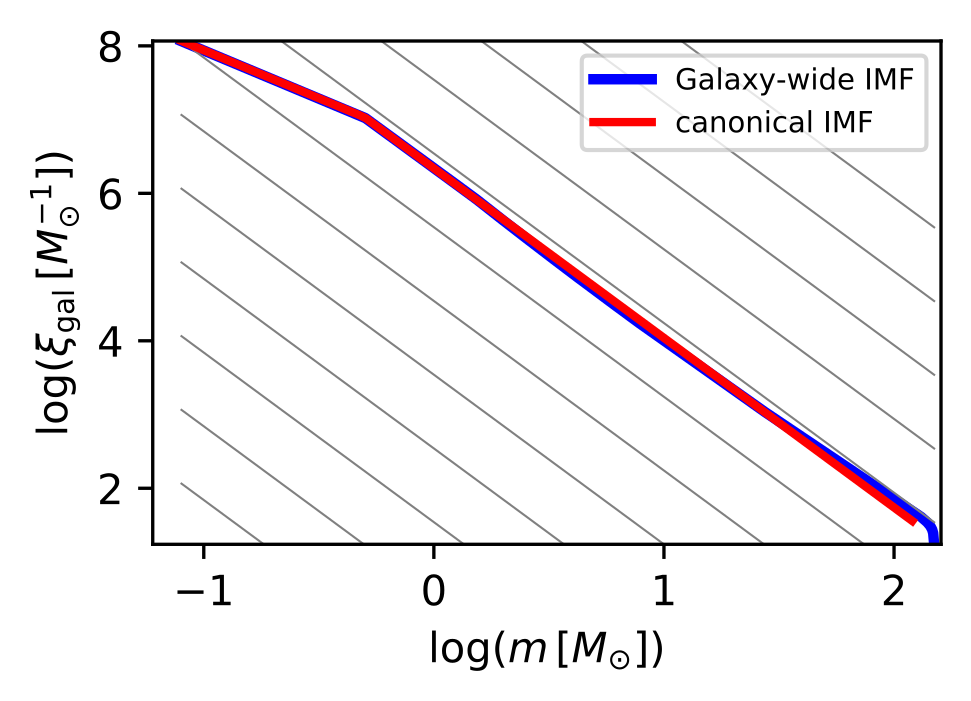
\includegraphics[width=\textwidth]{sfr1-feh0.png}
		\caption{SFR=1, $[\frac{Fe}{H}]=0$}
		\label{fig:2d-5dt}
	\end{subfigure}
	\begin{subfigure}[b]{0.4\textwidth}
	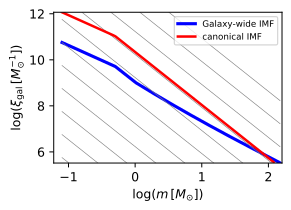
\includegraphics[width=\textwidth]{sfr1e4-feh0.png}
	\caption{SFR=$10^4$, $[\frac{Fe}{H}]=0$}
	\label{fig:2d-5dt}
	\end{subfigure}
	\begin{subfigure}[b]{0.45\textwidth}
%	\centering
	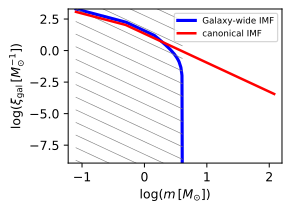
\includegraphics[width=\textwidth]{sfr1e-5-feh0.png}
	\caption{SFR=$10^{-5}$, $[\frac{Fe}{H}]=0$}
	\label{fig:2d-5dt}
	\end{subfigure}
	\caption{rebuild of A selection of IGIMF models which related to metalicity (in form of $[\frac{Fe}{H}$]=1,0,-3,-5)and SFR=$10^{-5},1,10^{4} \frac{M_{\odot}}{yr}$. All IMF models are
		normalized to the total stellar mass formed over $\delta t = 10 Myr$ to make the comparison with the canonical IMF (black dashed line in each panel)
		quantitative.}
	\label{fig:feh=0}
\end{figure}

\begin{figure}
	\centering
		\begin{subfigure}[b]{0.4\textwidth}
		%	\centering
		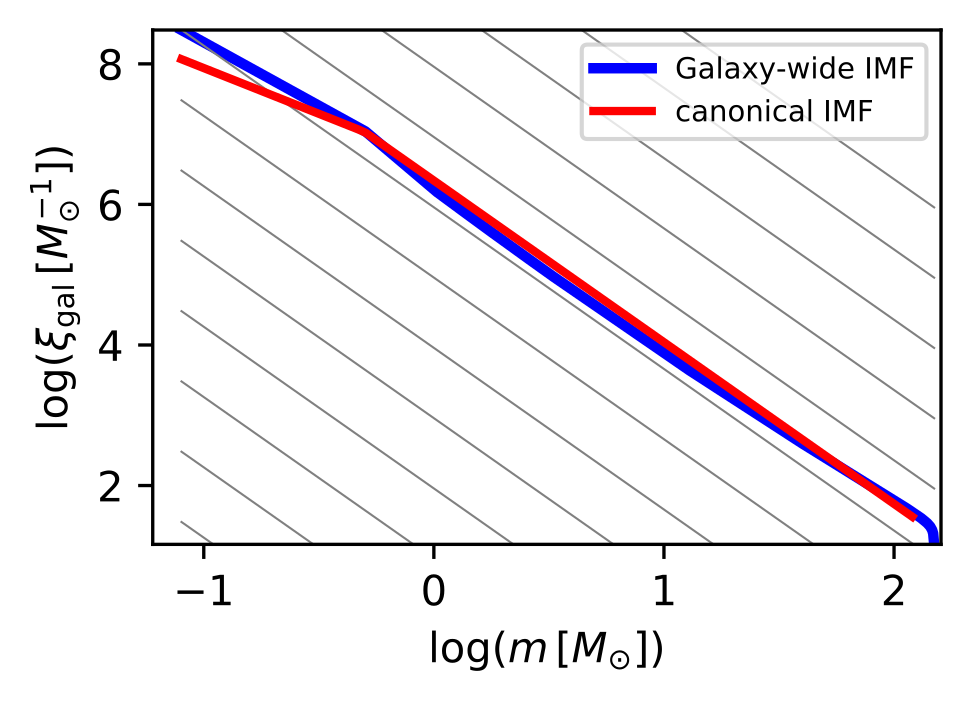
\includegraphics[width=\textwidth]{sfr1-feh1.png}
		\caption{SFR=$10^{0}$, $[\frac{Fe}{H}]=1$}
		\label{fig:s1e4-1}
	\end{subfigure}
	\begin{subfigure}[b]{0.4\textwidth}
		%	\centering
		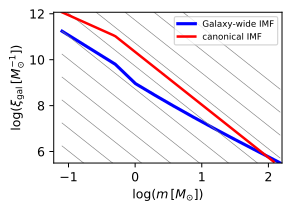
\includegraphics[width=\textwidth]{sfr1e4-feh1.png}
		\caption{SFR=$10^{4}$, $[\frac{Fe}{H}]=1$}
		\label{fig:s1e4-1}
	\end{subfigure}
\begin{subfigure}[b]{0.45\textwidth}
	%	\centering
	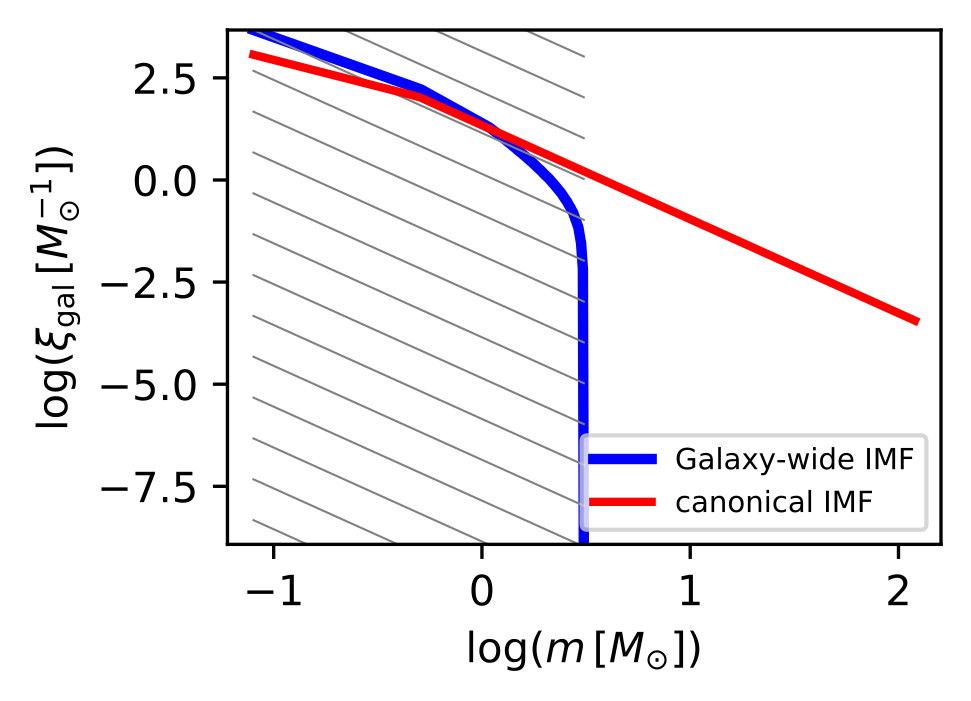
\includegraphics[width=\textwidth]{sfr1e-5-feh1.png}
	\caption{SFR=$10^{-5}$, $[\frac{Fe}{H}]=1$}
	\label{fig:s1e4-1}
\end{subfigure}
	\caption{rebuild of A selection of IGIMF models which related to metalicity (in form of $[\frac{Fe}{H}$]=1,0,-3,-5)and SFR=$10^{-5},1,10^{4} \frac{M_{\odot}}{yr}$. All IMF models are
	normalized to the total stellar mass formed over $\delta t = 10 Myr$ to make the comparison with the canonical IMF (black dashed line in each panel)
	quantitative.}
\label{fig:grid-sfr}
\end{figure}

\begin{figure}
	\centering
	\begin{subfigure}[b]{0.4\textwidth}
		%	\centering
		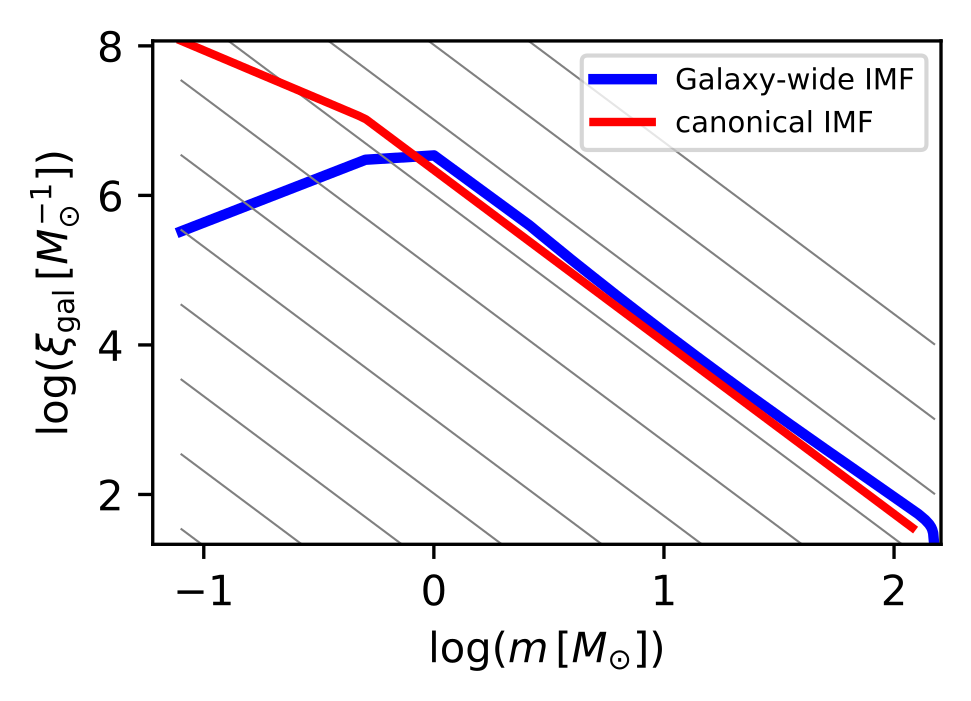
\includegraphics[width=\textwidth]{sfr1-feh-5.png}
		\caption{SFR=$10^{0}$, $[\frac{Fe}{H}]=-5$}
		\label{fig:s1e4-1}
	\end{subfigure}
	\begin{subfigure}[b]{0.4\textwidth}
		%\centering
		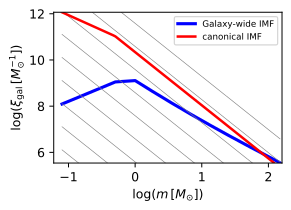
\includegraphics[width=\textwidth]{sfr1e4-feh-5.png}
		\caption{SFR=$10^{4}$, $[\frac{Fe}{H}]=-5$}
		\label{fig:2d-5dt}
	\end{subfigure}
	
	\begin{subfigure}[b]{0.45\textwidth}
		%\centering
		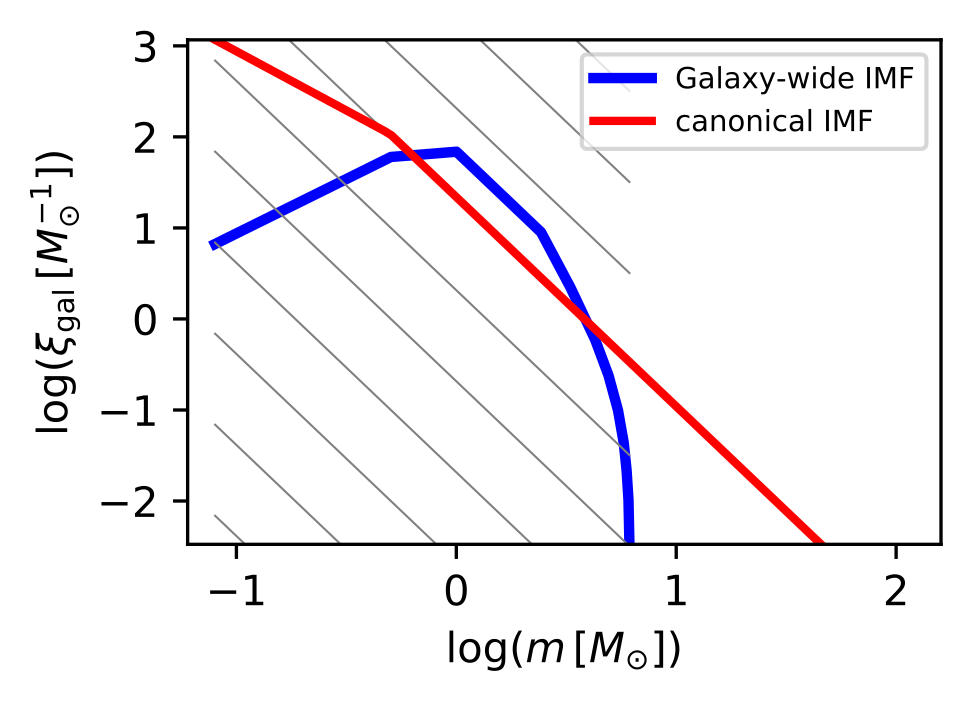
\includegraphics[width=\textwidth]{sfr1e-5-feh-5.png}
		\caption{SFR=$10^{-5}$, $[\frac{Fe}{H}]=-5$}
		\label{fig:2d-5dt}
	\end{subfigure}
	\caption{rebuild of A selection of IGIMF models which related to metalicity (in form of $[\frac{Fe}{H}$]=1,0,-3,-5)and SFR=$10^{-5},1,10^{4} \frac{M_{\odot}}{yr}$. All IMF models are
		normalized to the total stellar mass formed over $\delta t = 10 Myr$ to make the comparison with the canonical IMF (black dashed line in each panel)
		quantitative.}
	\label{fig:feh-5}
\end{figure}
\begin{figure}
	\centering
	\begin{subfigure}[b]{0.4\textwidth}
		%	\centering
		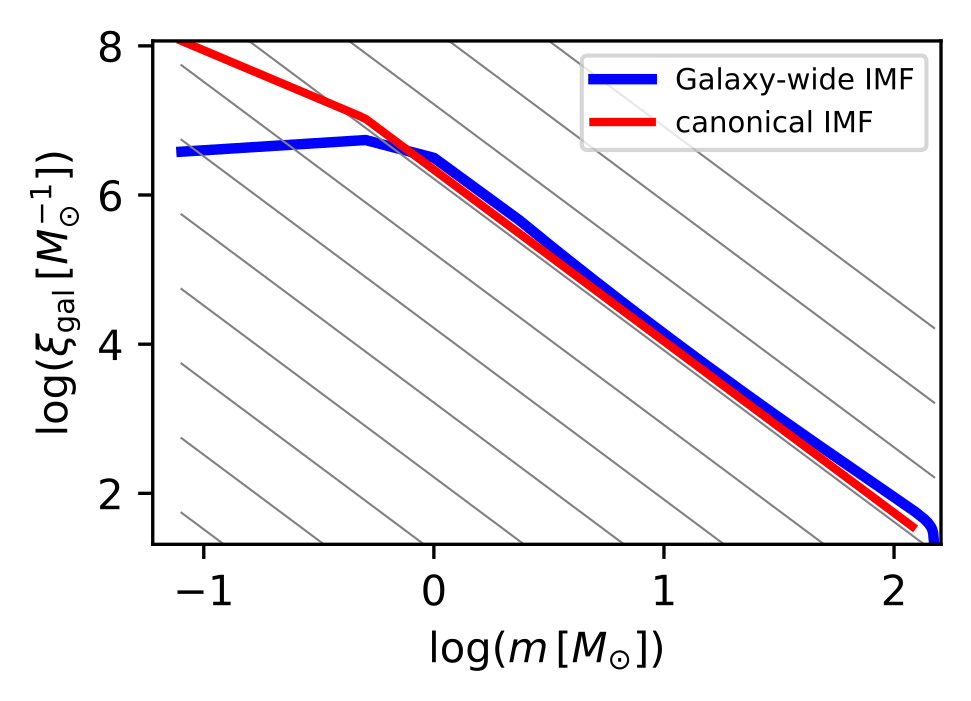
\includegraphics[width=\textwidth]{sfr1-feh-3.png}
		\caption{SFR=$10^{0}$, $[\frac{Fe}{H}]=-3$}
		\label{fig:s1e4-1}
	\end{subfigure}
	\begin{subfigure}[b]{0.4\textwidth}
		%\centering
		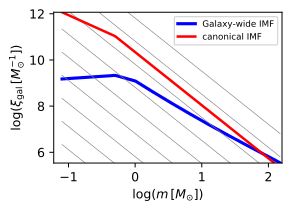
\includegraphics[width=\textwidth]{sfr1e4-feh-3.png}
		\caption{SFR=$10^{4}$, $[\frac{Fe}{H}]=-3$}
		\label{fig:2d-5dt}
	\end{subfigure}
	
	\begin{subfigure}[b]{0.45\textwidth}
		%\centering
		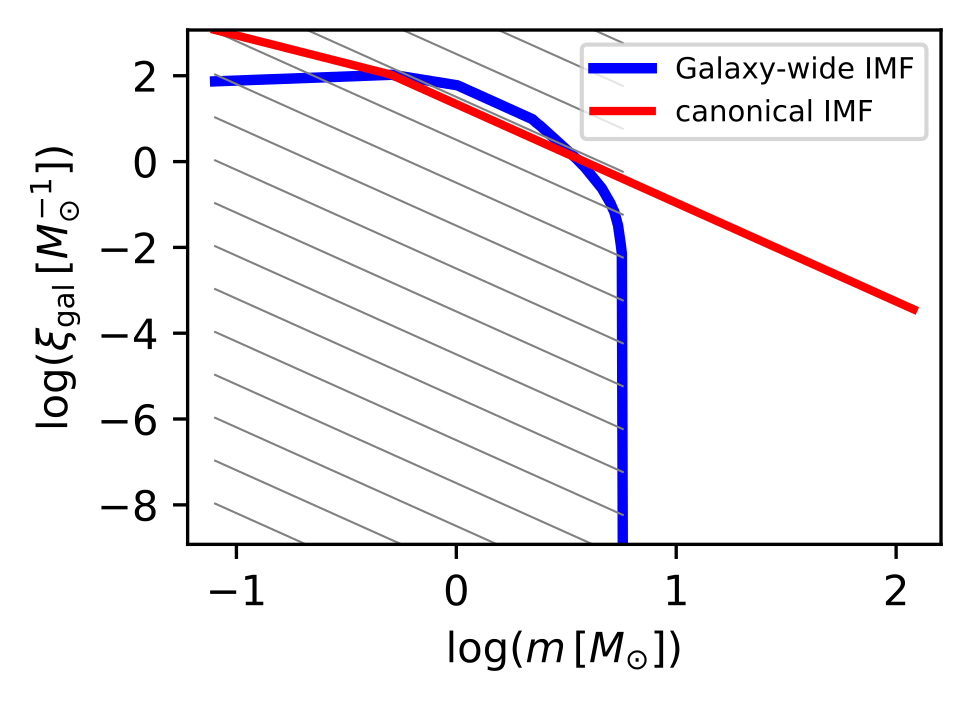
\includegraphics[width=\textwidth]{sfr1e-5-feh-3.png}
		\caption{SFR=$10^{-5}$, $[\frac{Fe}{H}]=-3$}
		\label{fig:2d-5dt}
	\end{subfigure}
	\caption{rebuild of A selection of IGIMF models which related to metalicity (in form of $[\frac{Fe}{H}$]=-3)and SFR=$10^{-5},1,10^{4} \frac{M_{\odot}}{yr}$. All IMF models are
		normalized to the total stellar mass formed over $\delta t = 10 Myr$ to make the comparison with the canonical IMF (black dashed line in each panel)
		quantitative.}
	\label{fig:feh-3}
\end{figure}


\section{}

\section*{title}


\section{Two-dimensional diffusion equation}


\section{Results for two-dimensional heat equation}
\subsection{The case of constant diffusion coefficient}
In the previous sections we have found that the CG algorithm are much more efficient than the direct methods such as LU decomposition, so all the simulation for the two-dimentional equation have been done using CG method.
\\
\begin{figure}[ht]\centering
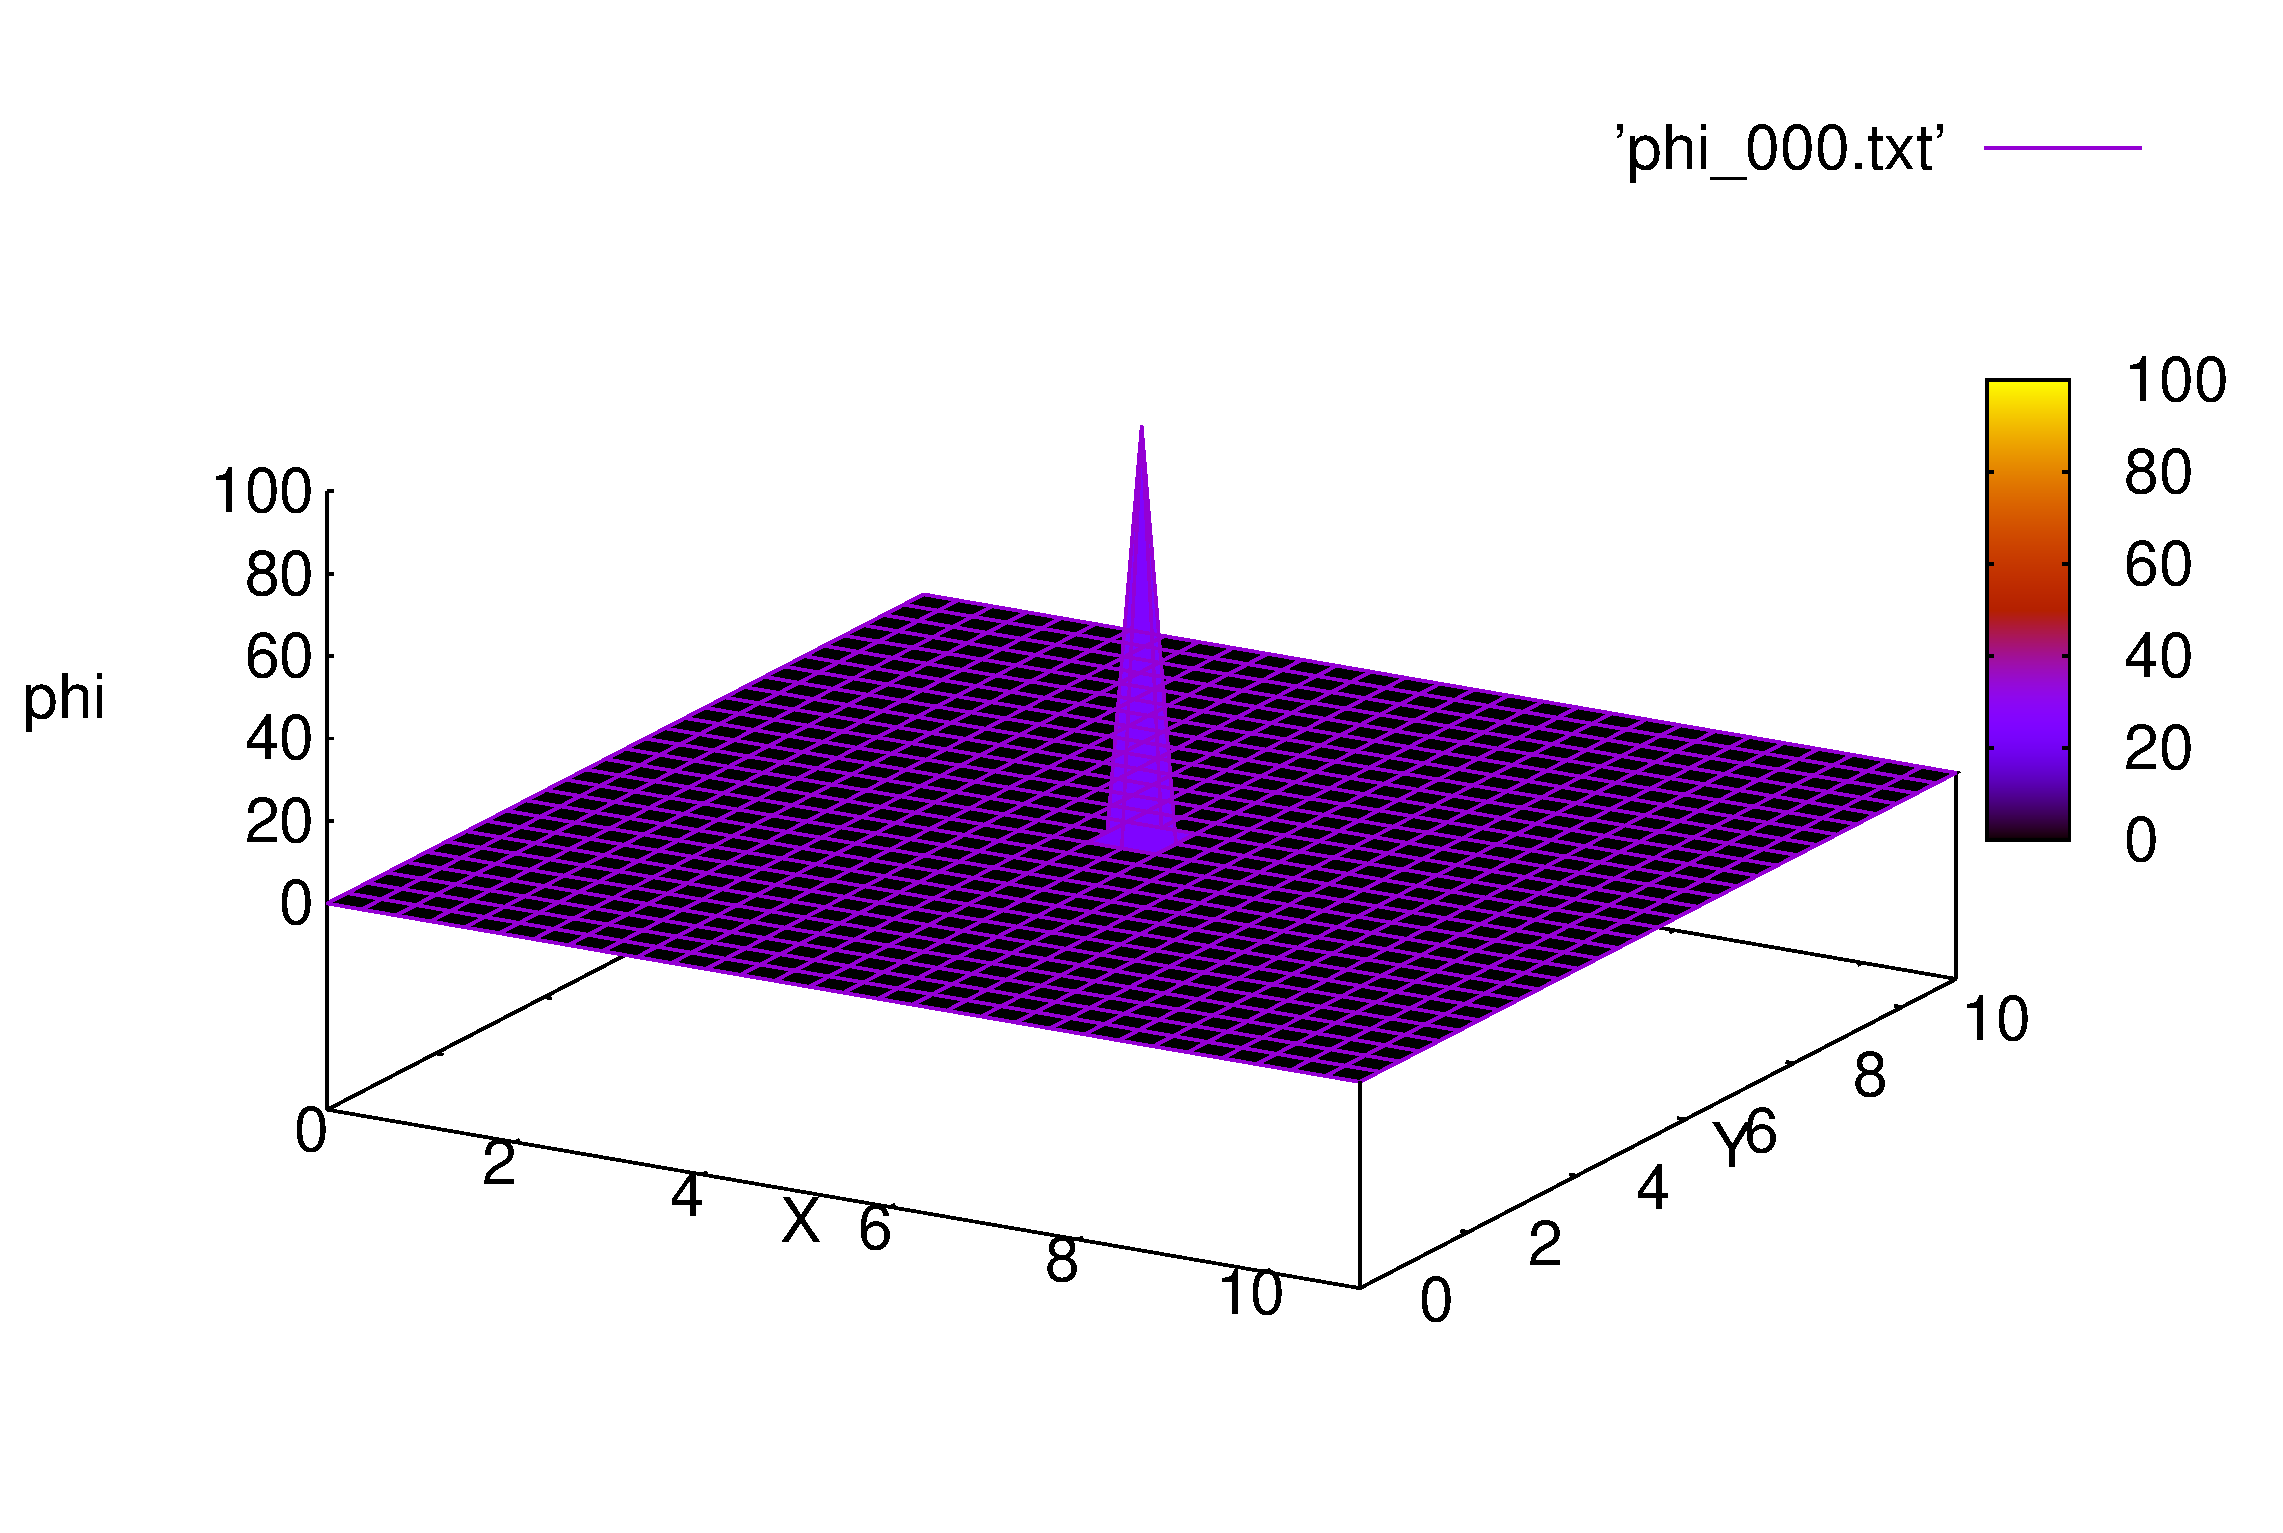
\includegraphics[width=\linewidth]{2DSimplefig/00}
\caption{initial condition for the 2D heat problem}
\label{fig:2d-initial_condition}
\end{figure}


%For the next step you will get figure \ref{fig:2d-1dt}.

%\begin{figure}[ht]\centering
%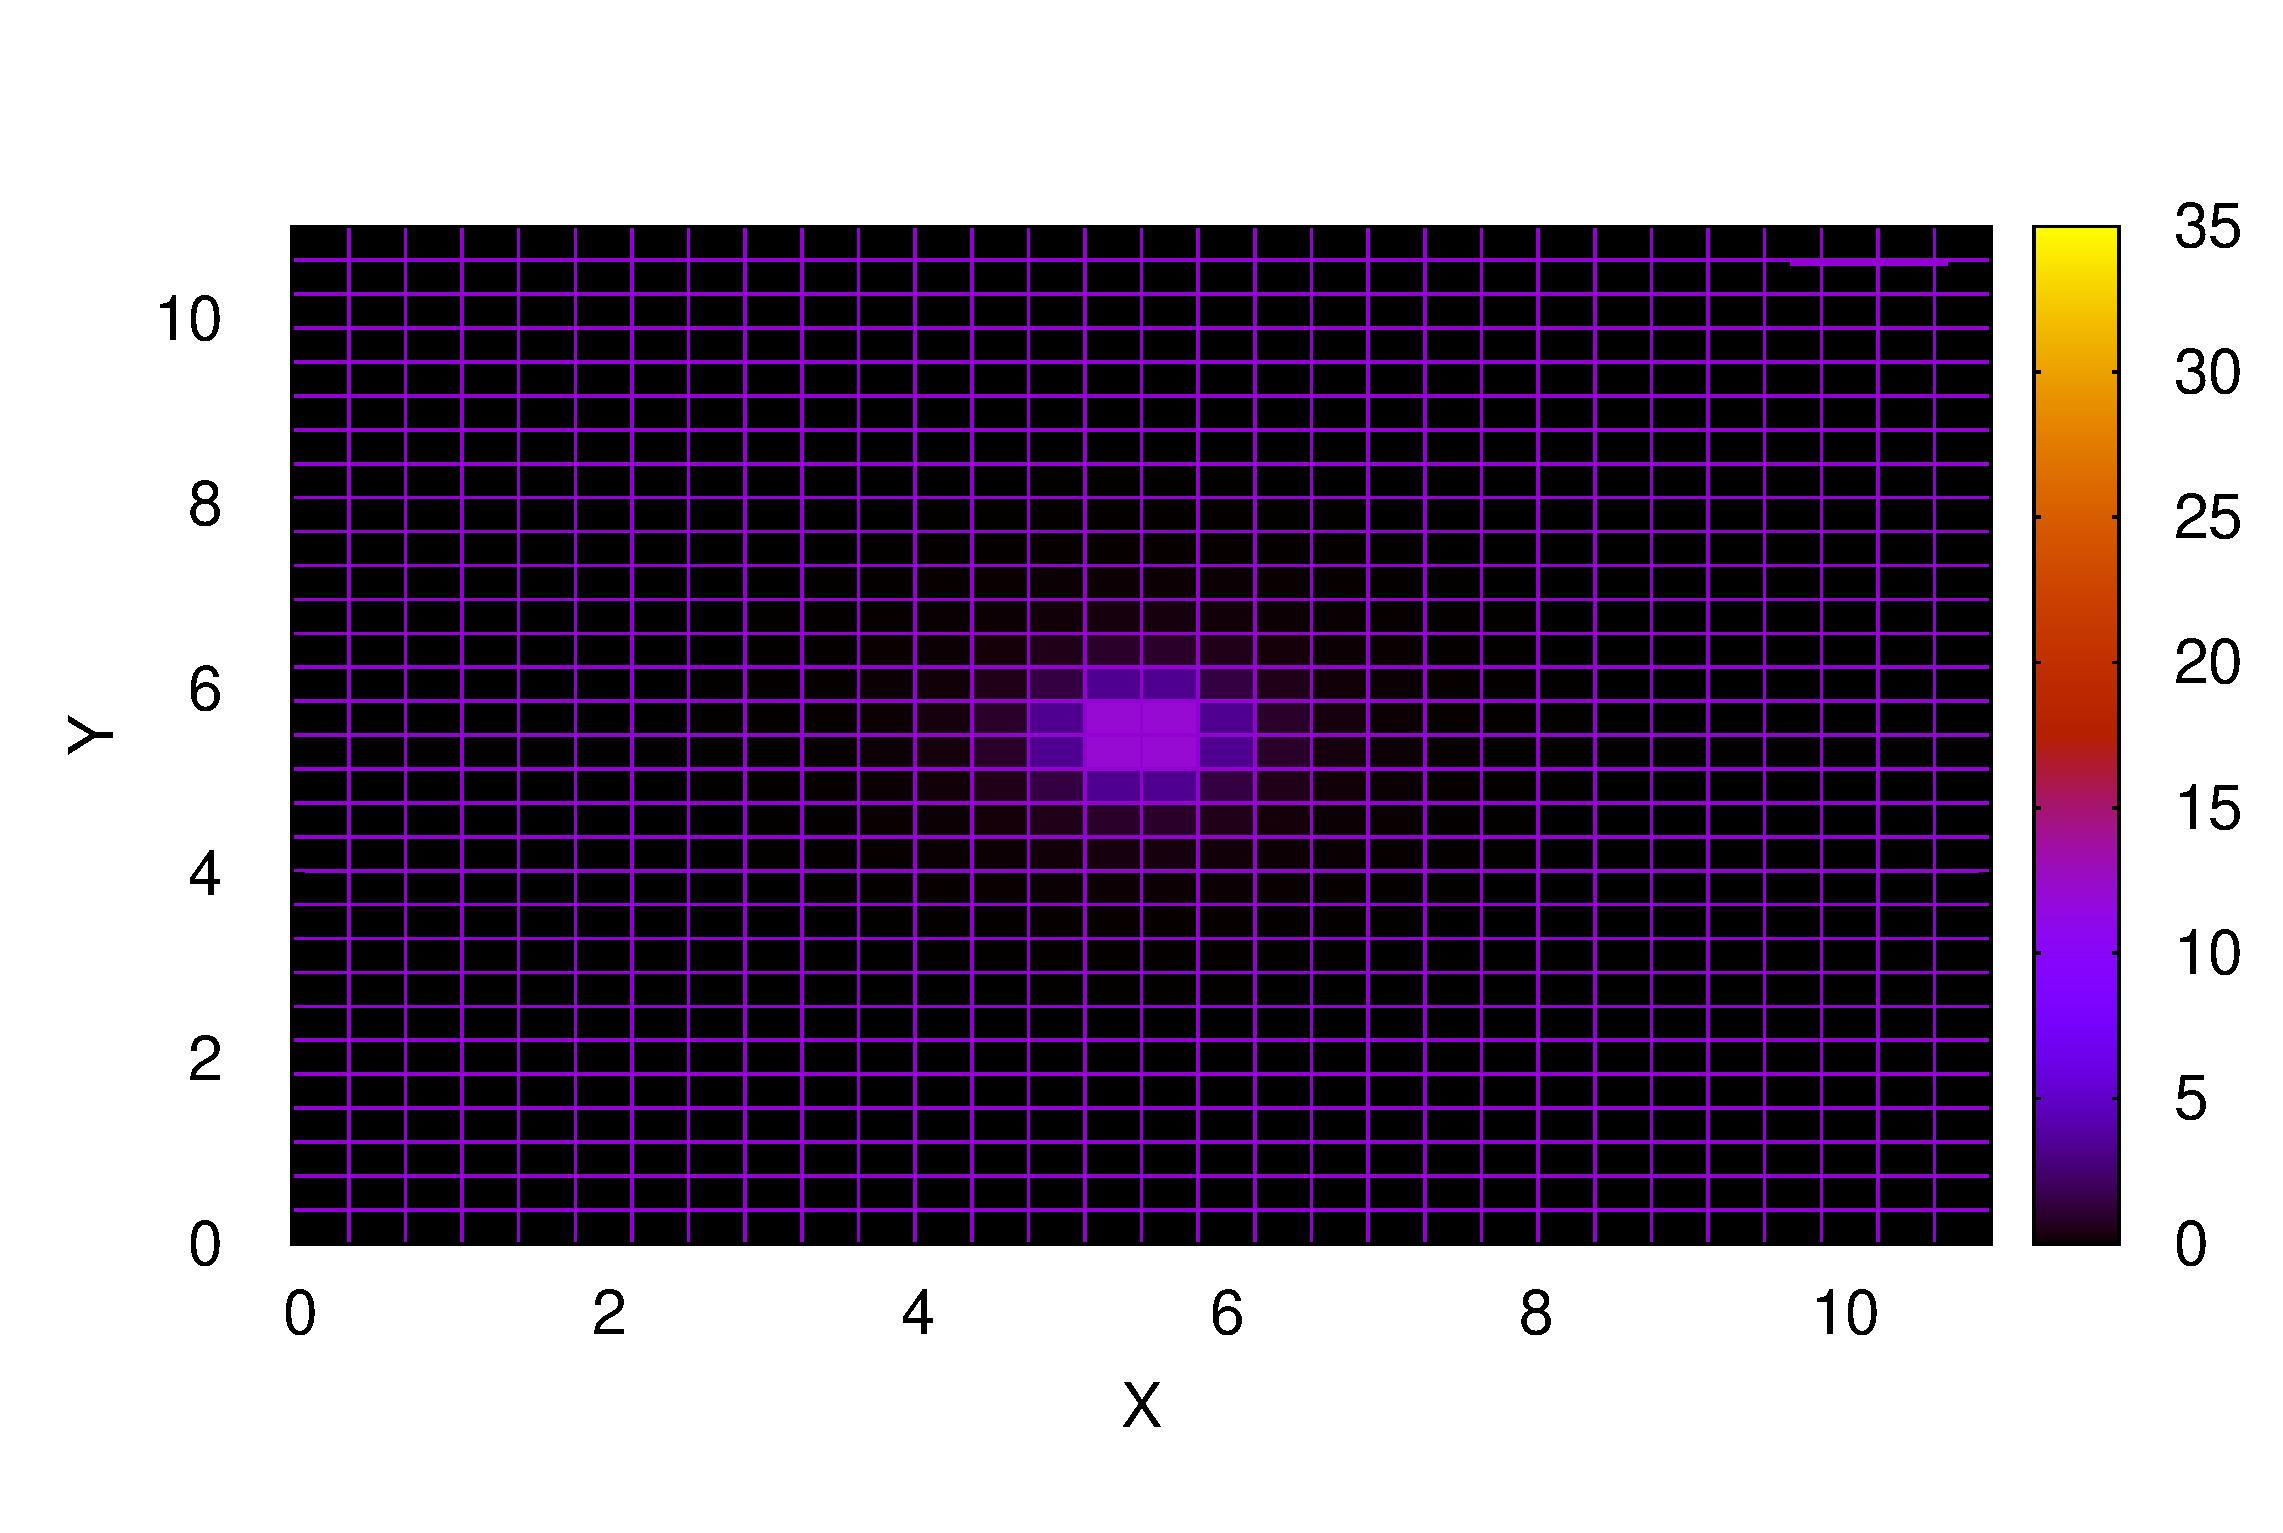
\includegraphics[width=\linewidth]{2DSimplefig/01_map}
%\caption{First step for the 2D heat problem}
%\label{fig:2d-1dt}
%\end{figure}

After 10 steps we will have figure \ref{fig:2d-10dt}. There is also an animation accessible at: \\
  \texttt{http://www.github.com/}. \\


\begin{figure}
     \centering
     \begin{subfigure}[b]{0.5\textwidth}
         \centering
         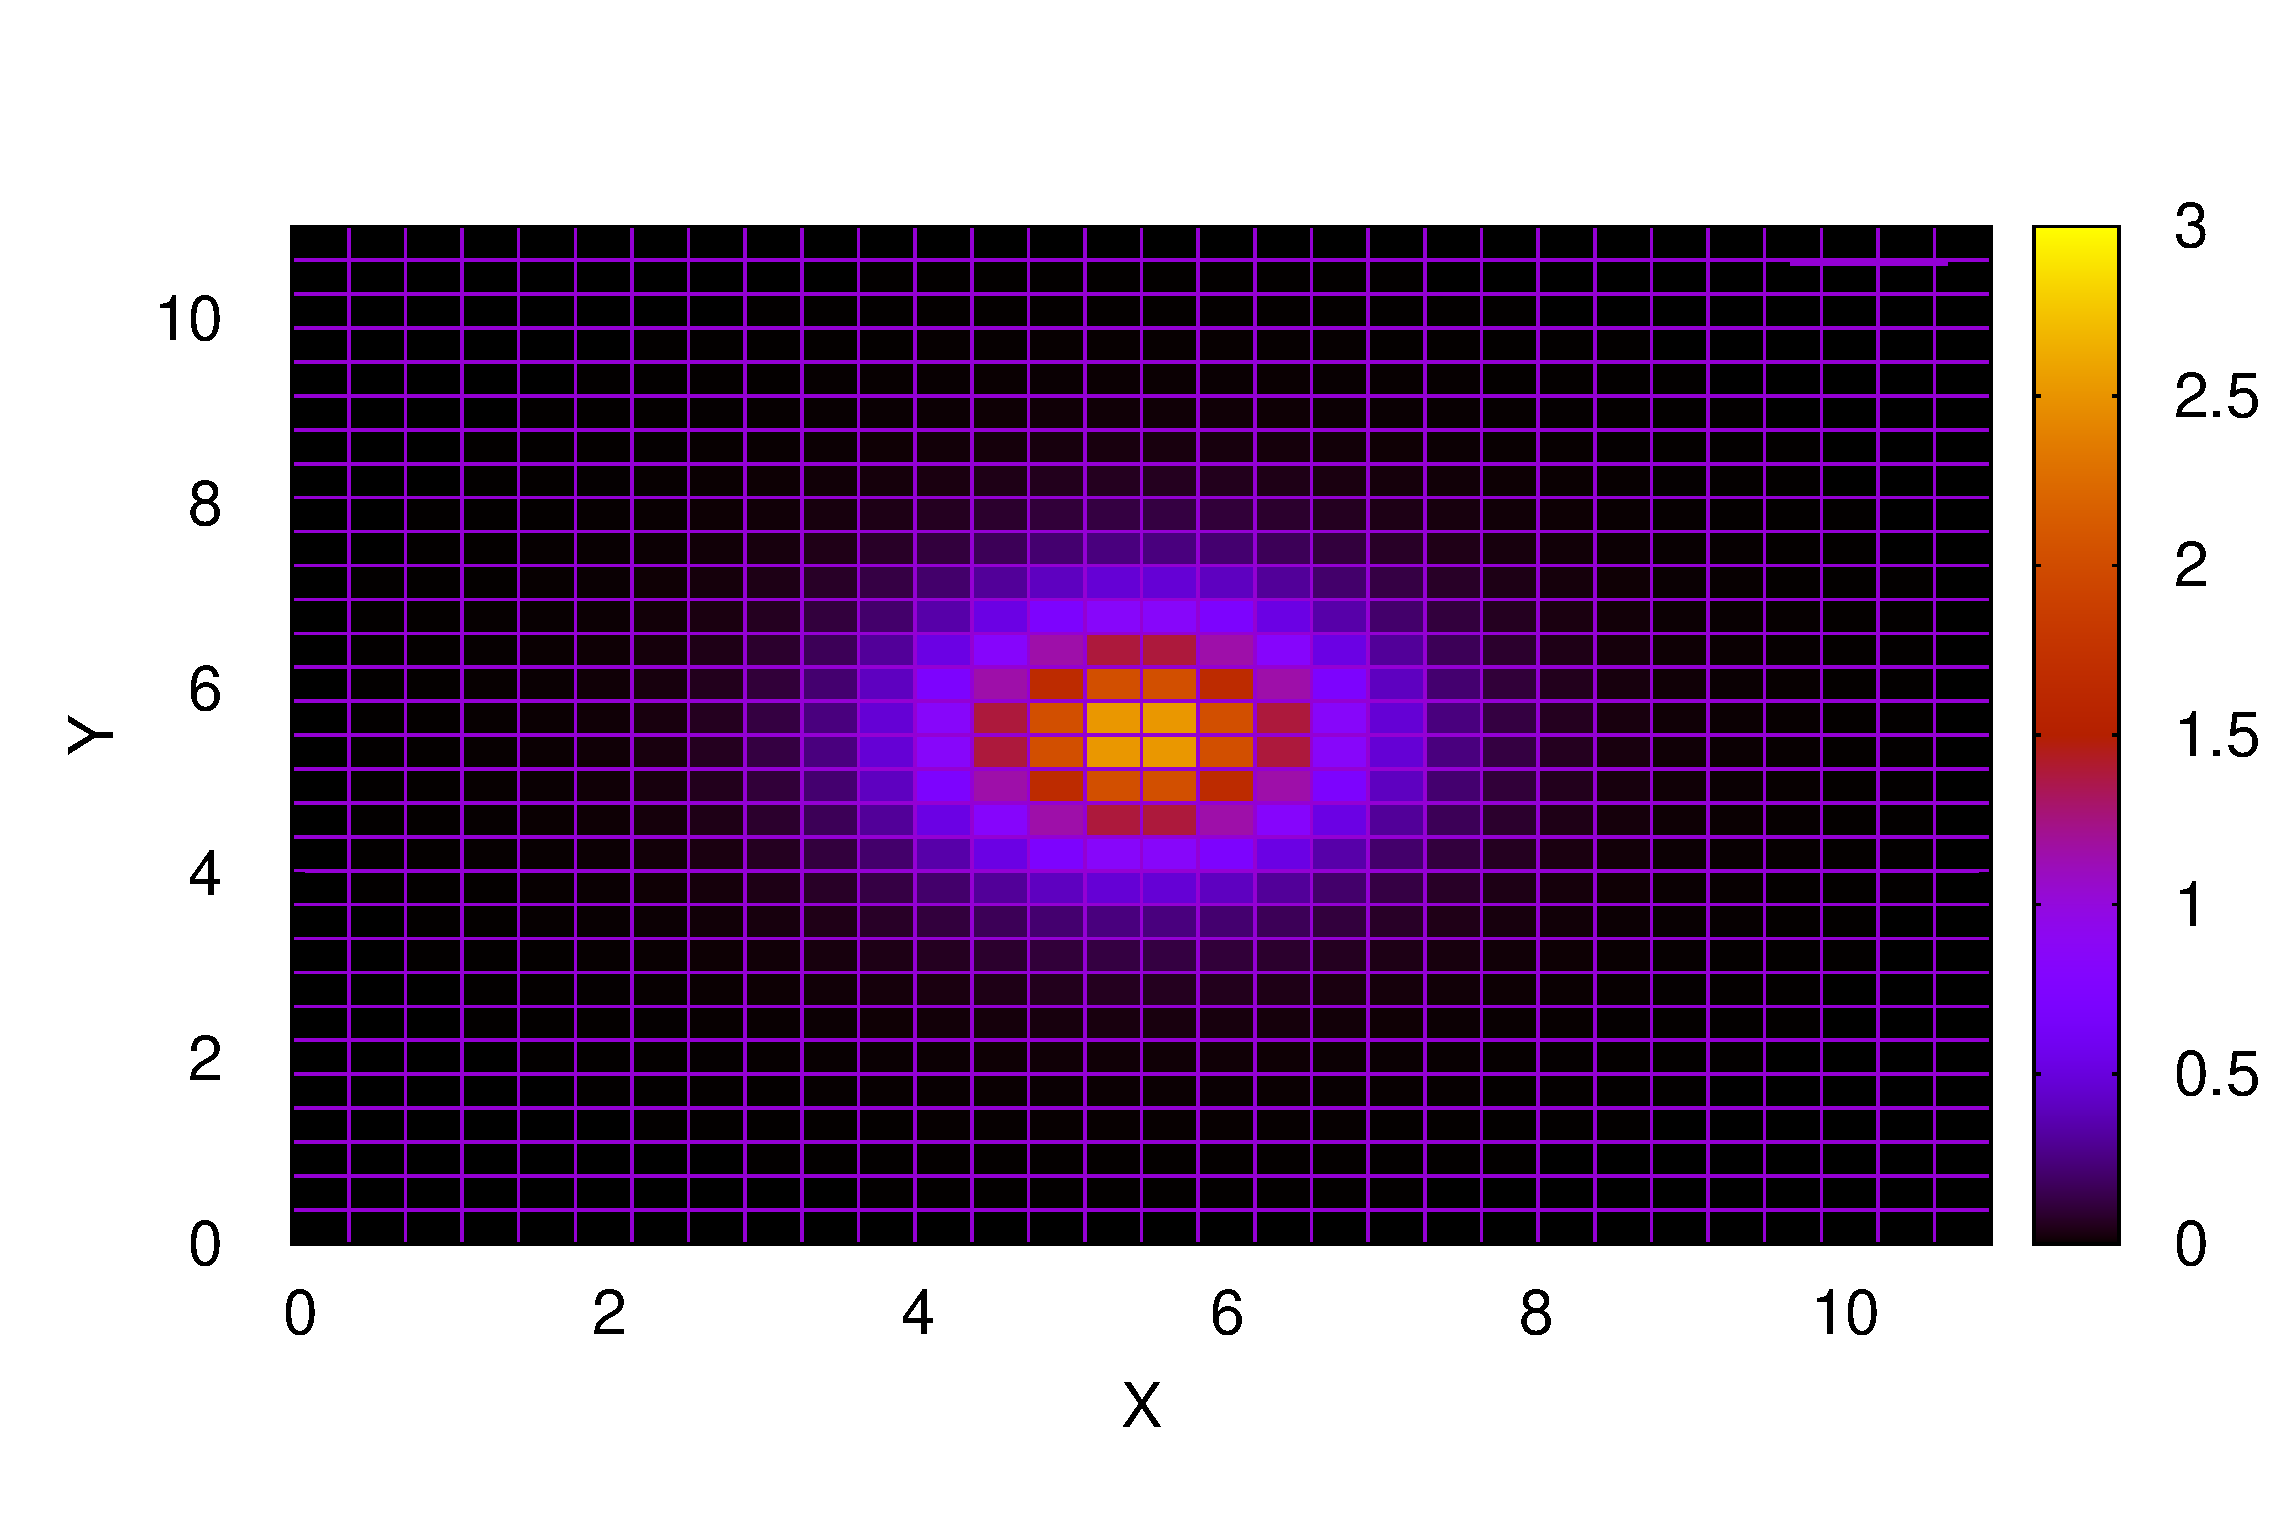
\includegraphics[width=\textwidth]{2DSimplefig/05_map}
		\caption{the heat distribution map after 5 timesteps for the 2D heat problem}
		\label{fig:2d-5dt}
     \end{subfigure}
     \hfill
	\centering
     \begin{subfigure}[b]{0.5\textwidth}
         \centering
         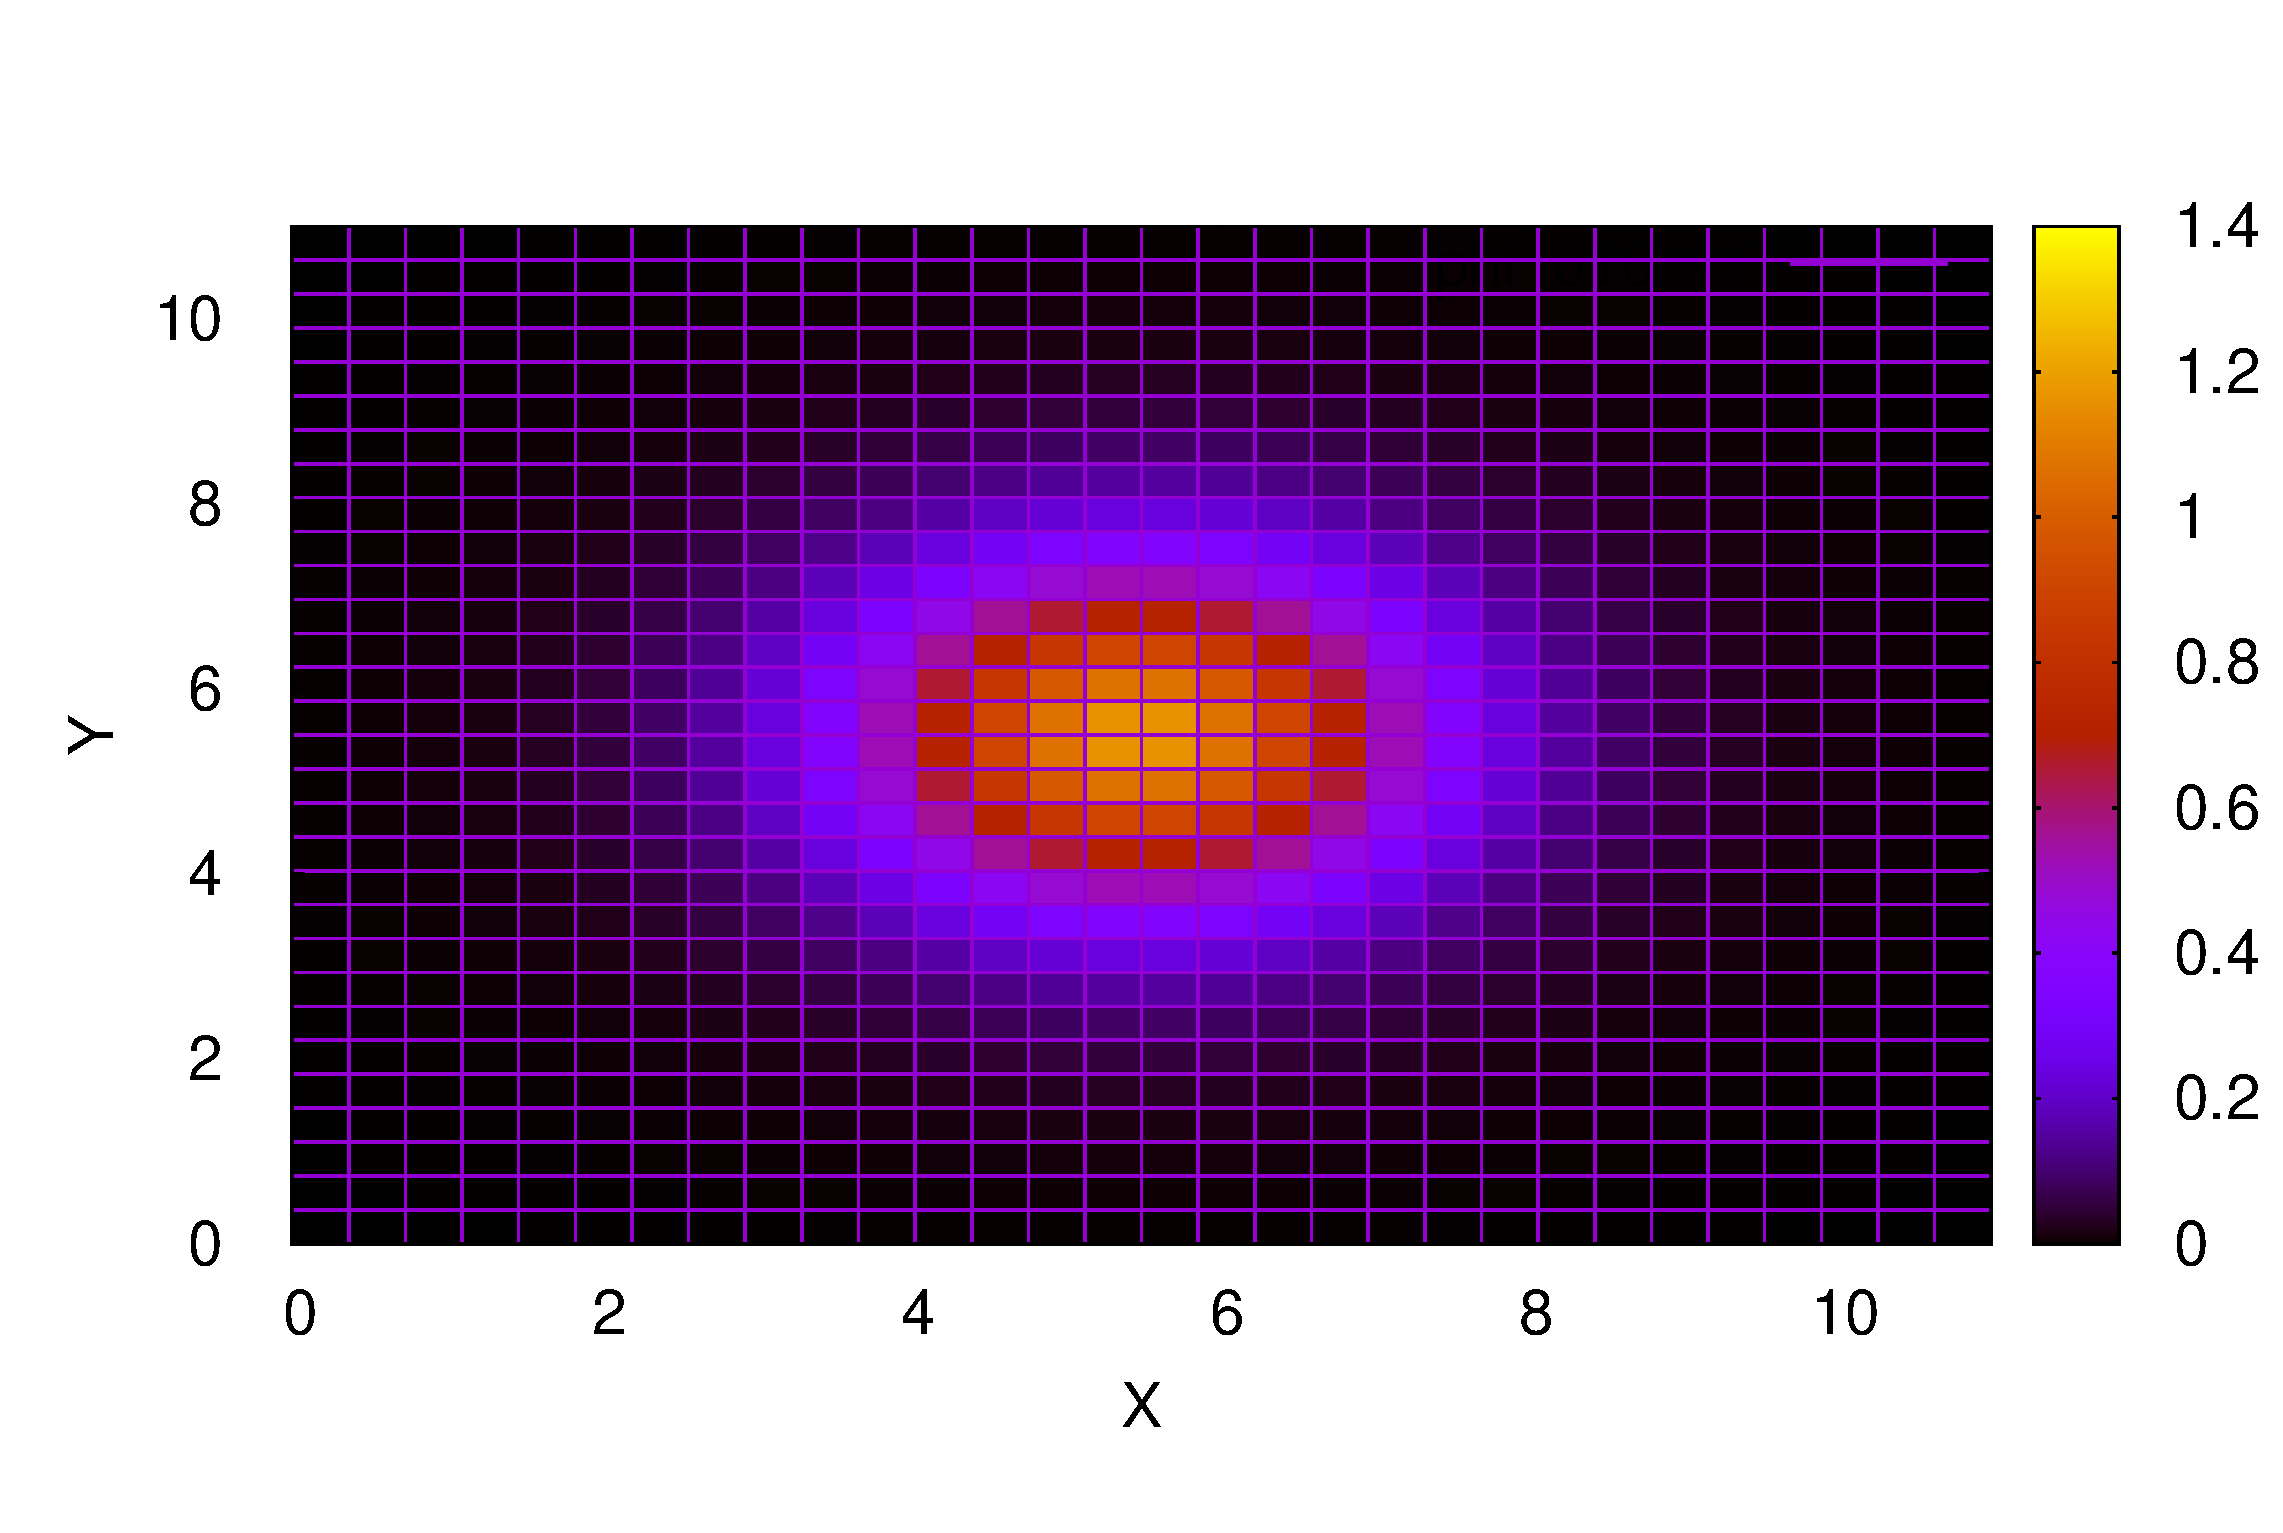
\includegraphics[width=\textwidth]{2DSimplefig/10_map}
		\caption{the heat distribution map after 10 timesteps for the 2D heat problem}
		\label{fig:2d-10dt}
     \end{subfigure}
     \hfill     
        \caption{solving two-dimensional heat equation using CG method.}
        \label{fig:2d-CG}
\end{figure}



In this case (constant diffusion coefficient), it is clear that the diffusion process is symmetric.
 \\

\subsection{The case of random diffusion coefficient}
The initial conditions of this case is the same as the initial condition for the constant diffusion coefficient (figure \ref{fig:2d-initial_condition}). 
\\

\begin{figure}
     \centering
     \begin{subfigure}[b]{0.45\textwidth}
         \centering
         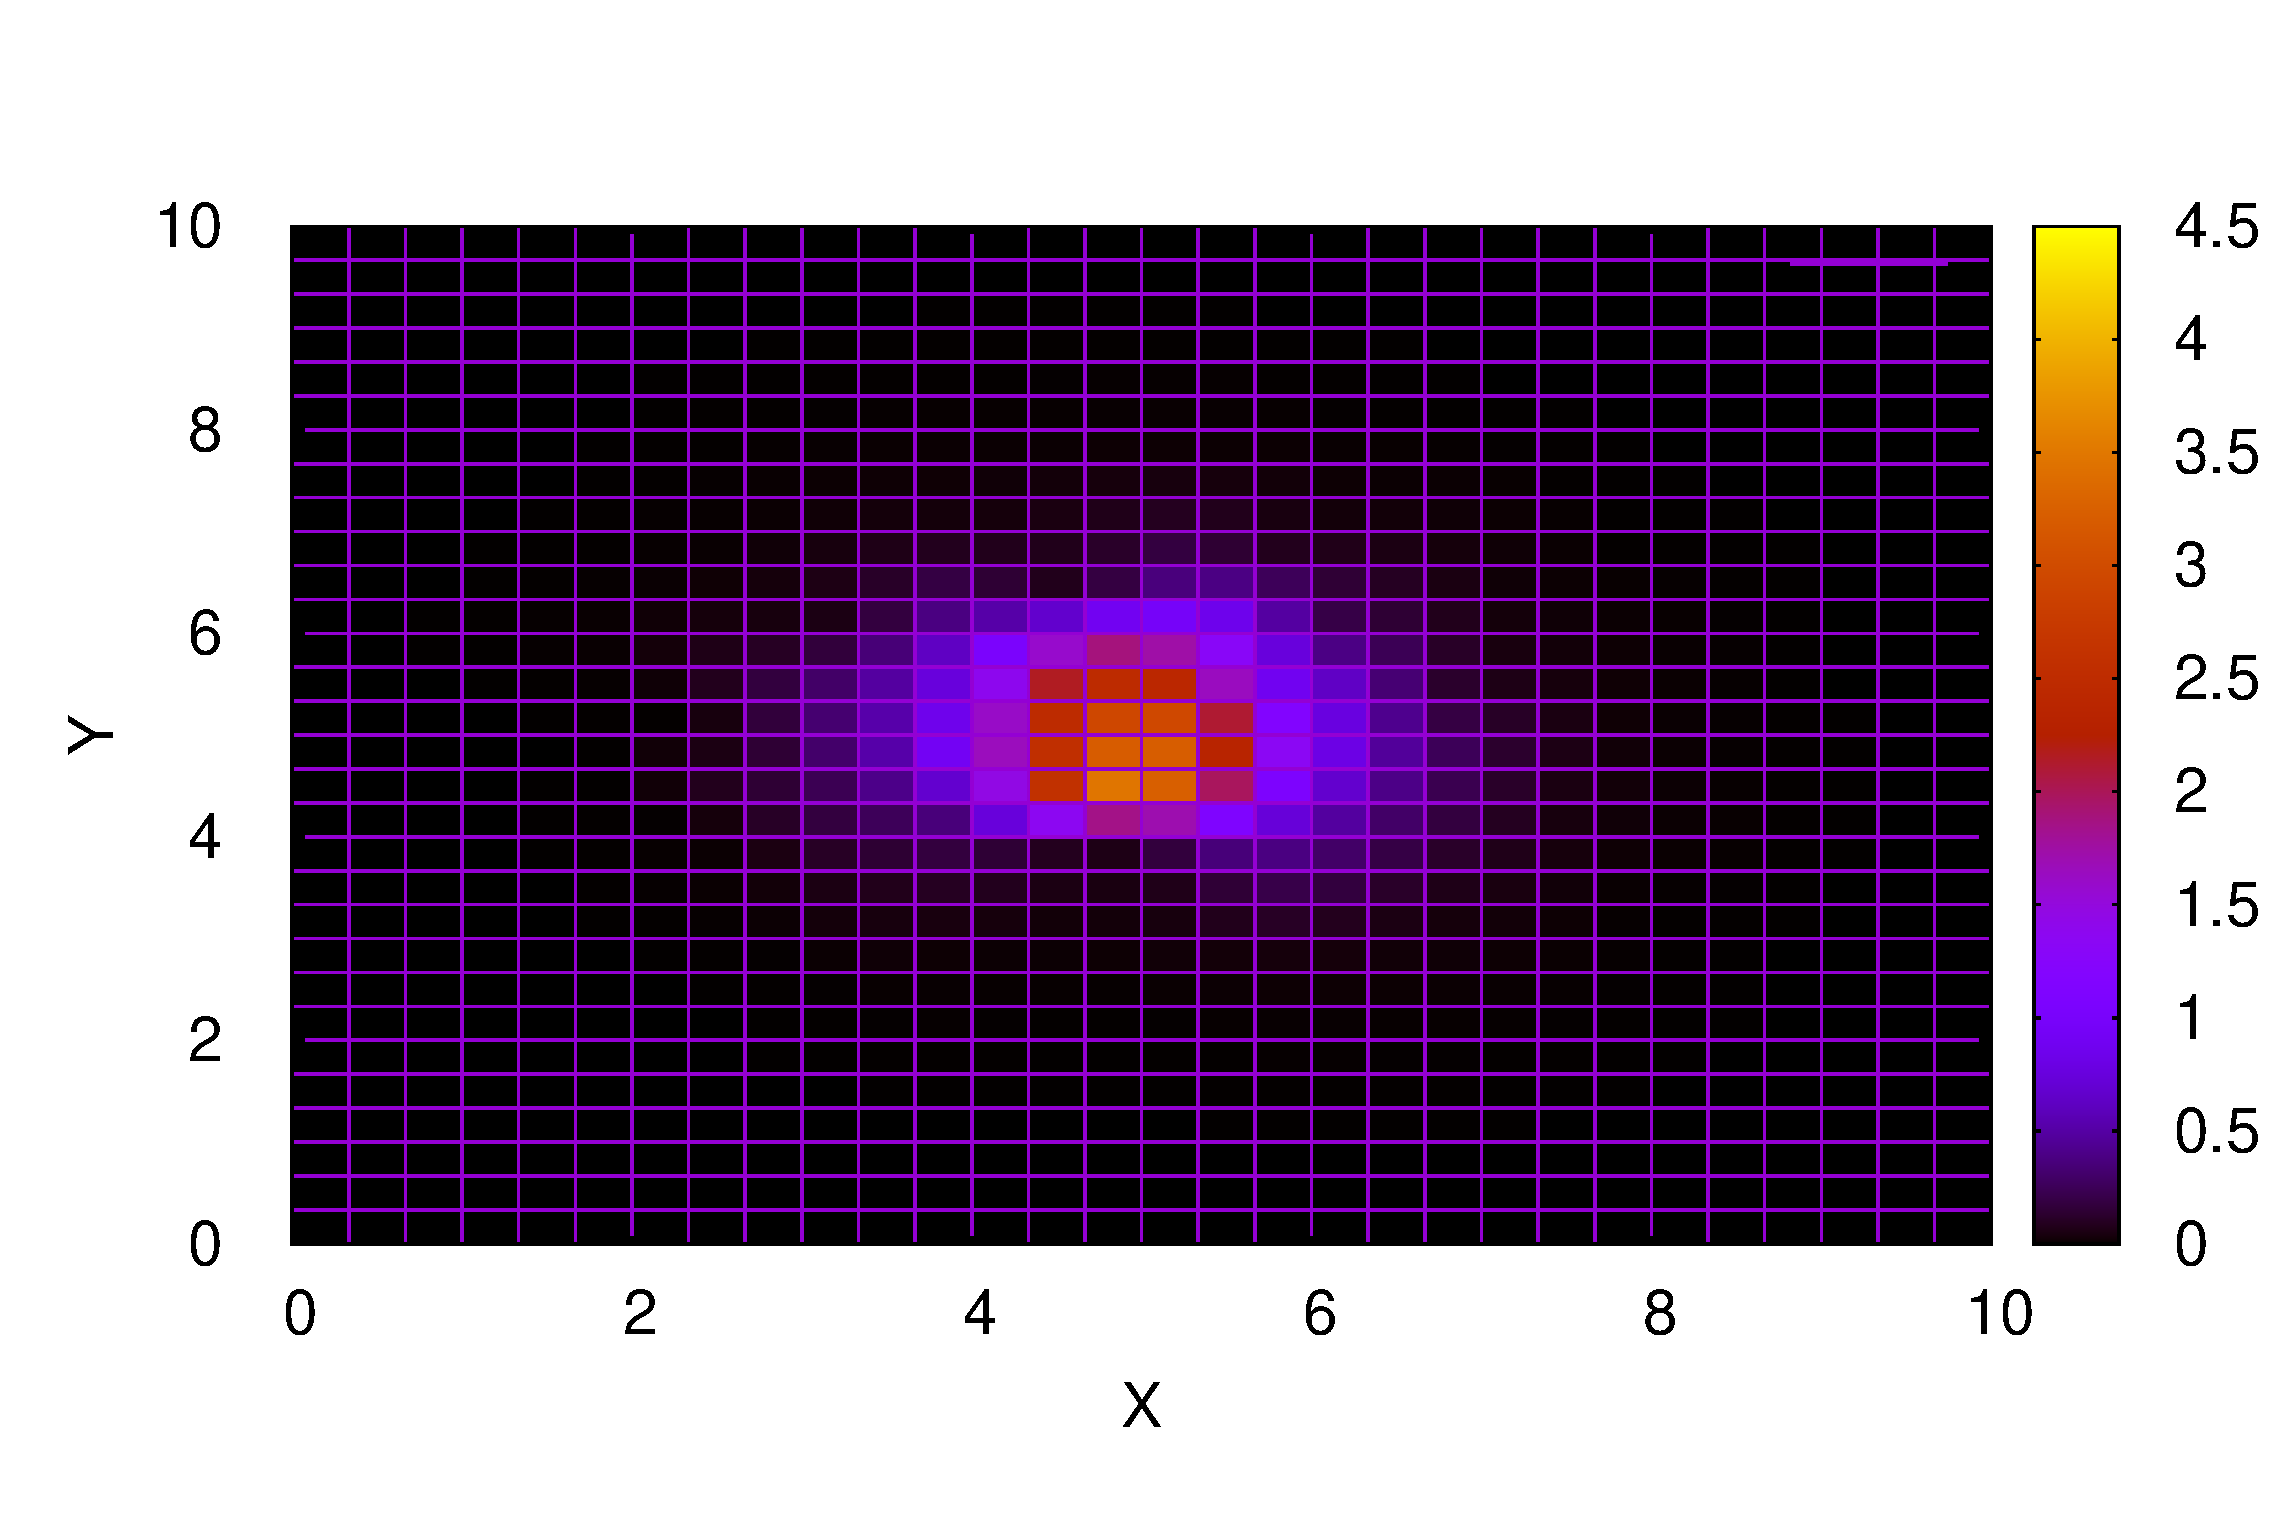
\includegraphics[width=\textwidth]{2DRandomDfig/05_map}
		\caption{the heat distribution map after 5 timesteps for the 2D heat problem}
		\label{fig:2d-randomD-5dt-map}
     \end{subfigure}
     \hfill
	\centering
     \begin{subfigure}[b]{0.45\textwidth}
         \centering
         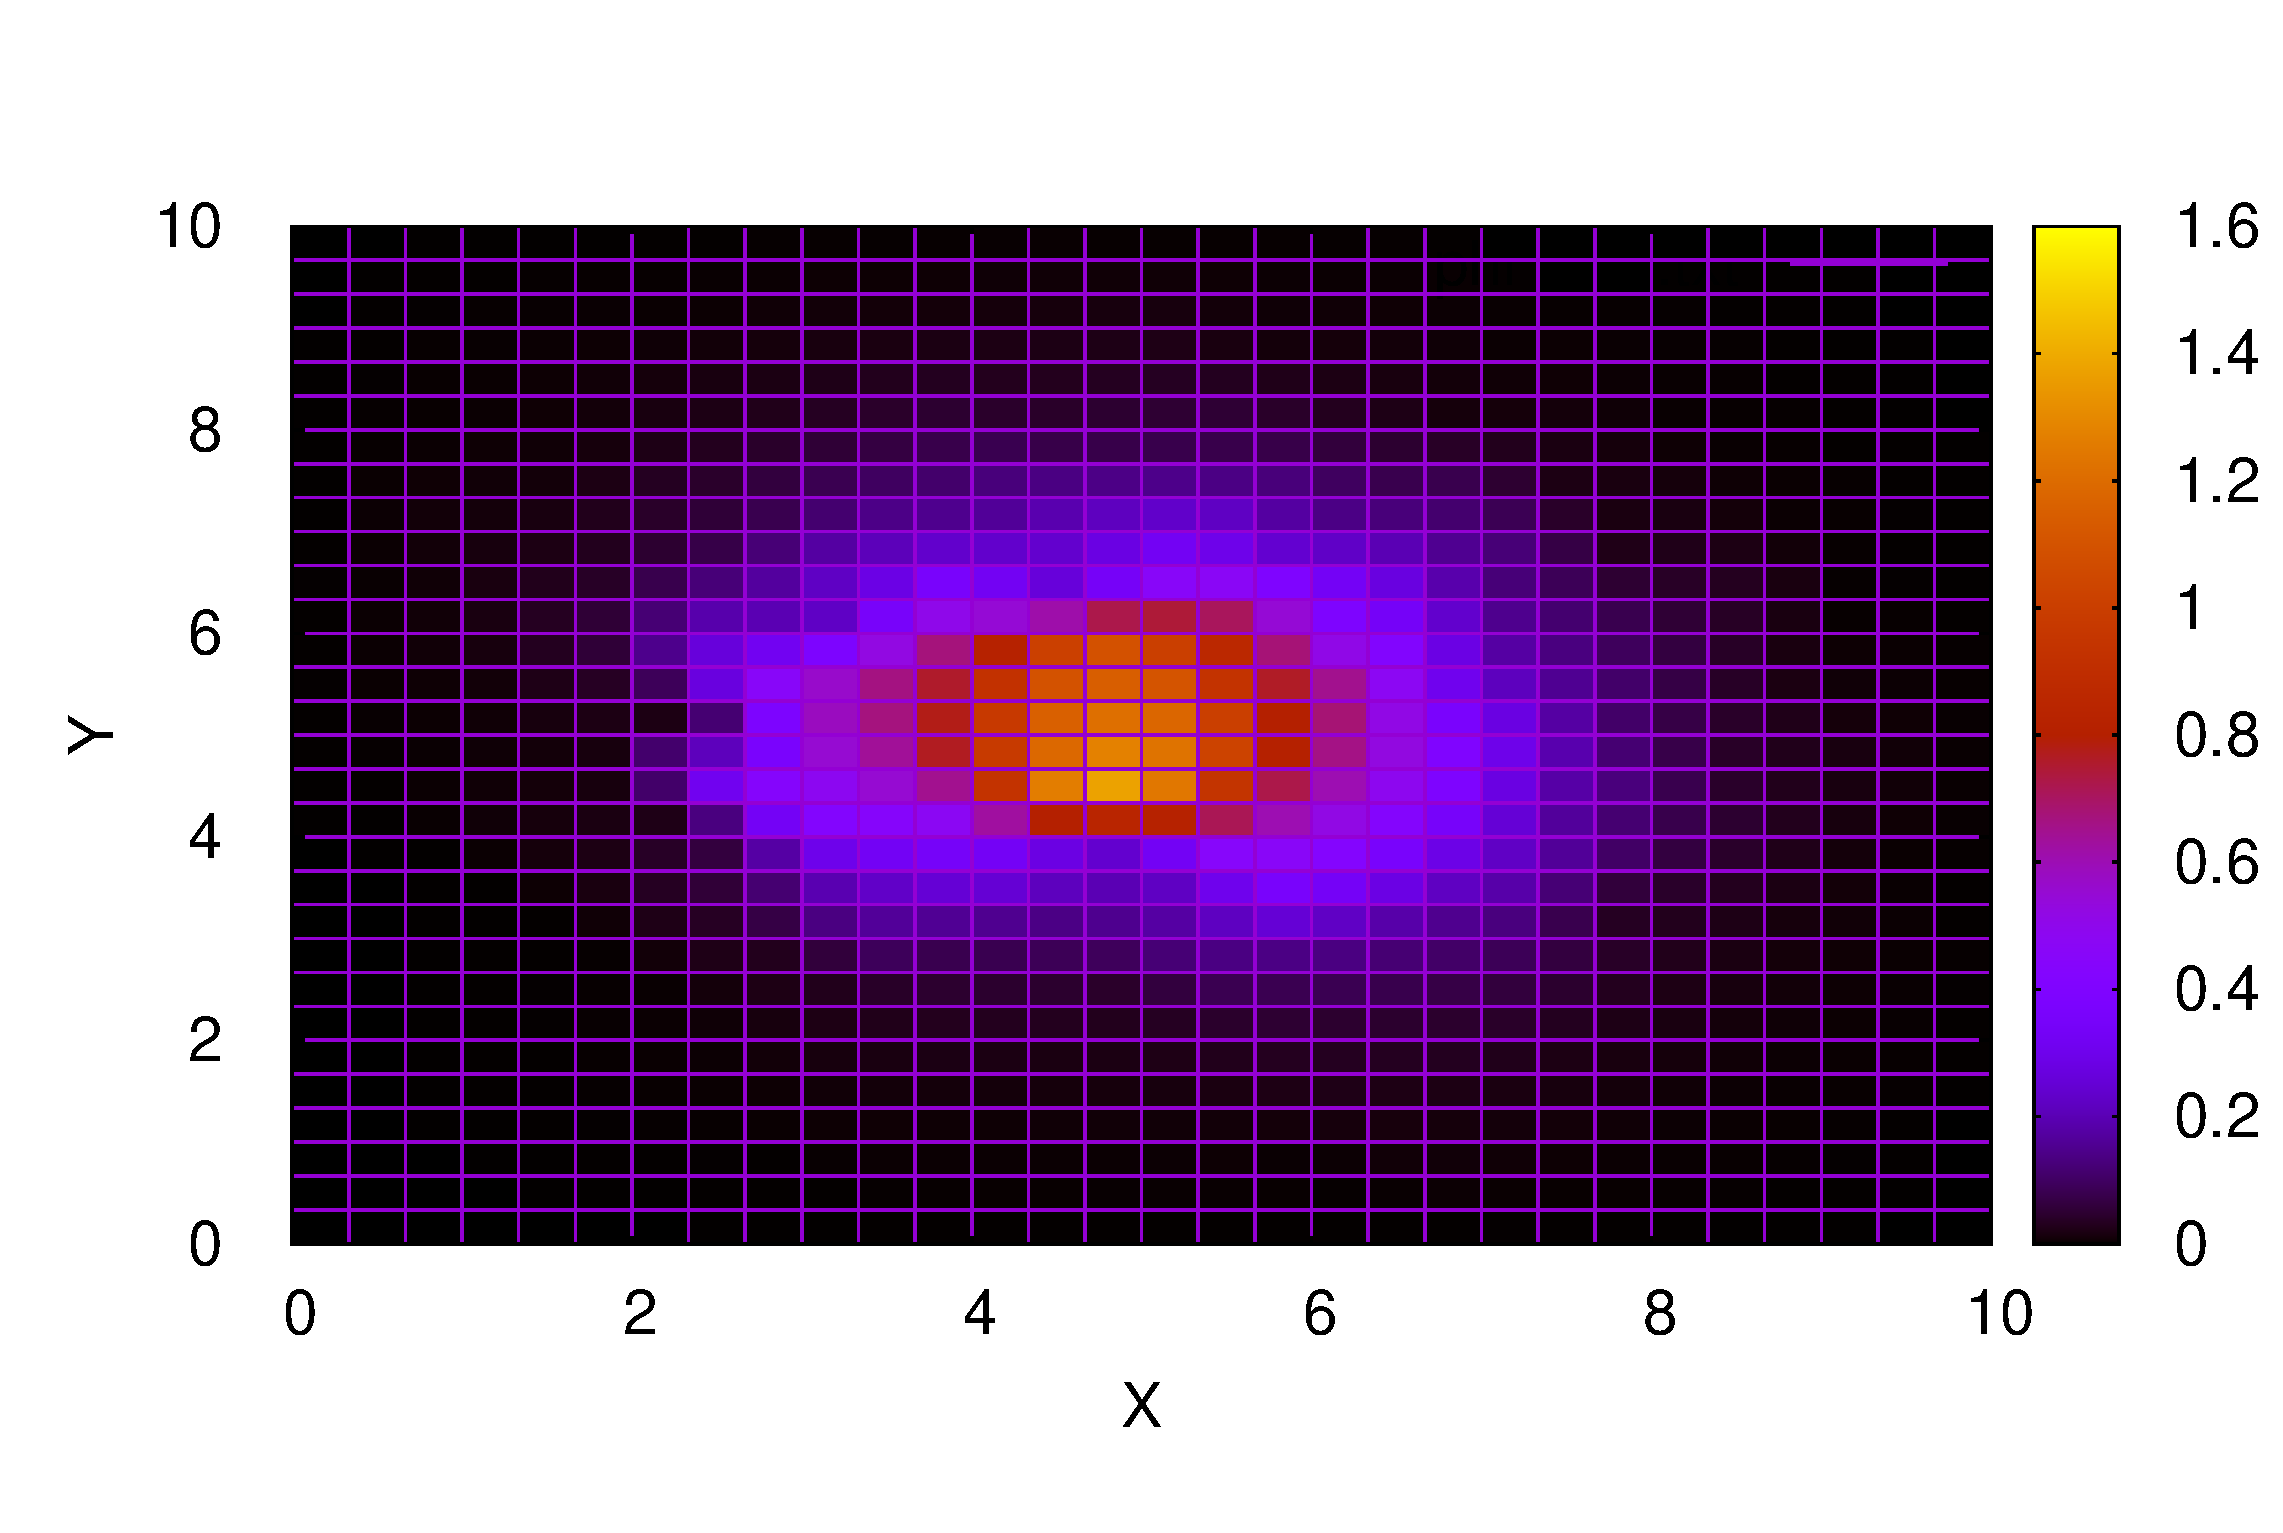
\includegraphics[width=\textwidth]{2DRandomDfig/15_map}
		\caption{the heat distribution map after 15 timesteps for the 2D heat problem}
		\label{fig:2d-randomD-15dt-map}
     \end{subfigure}
     \hfill     
          \begin{subfigure}[b]{0.45\textwidth}
         \centering
         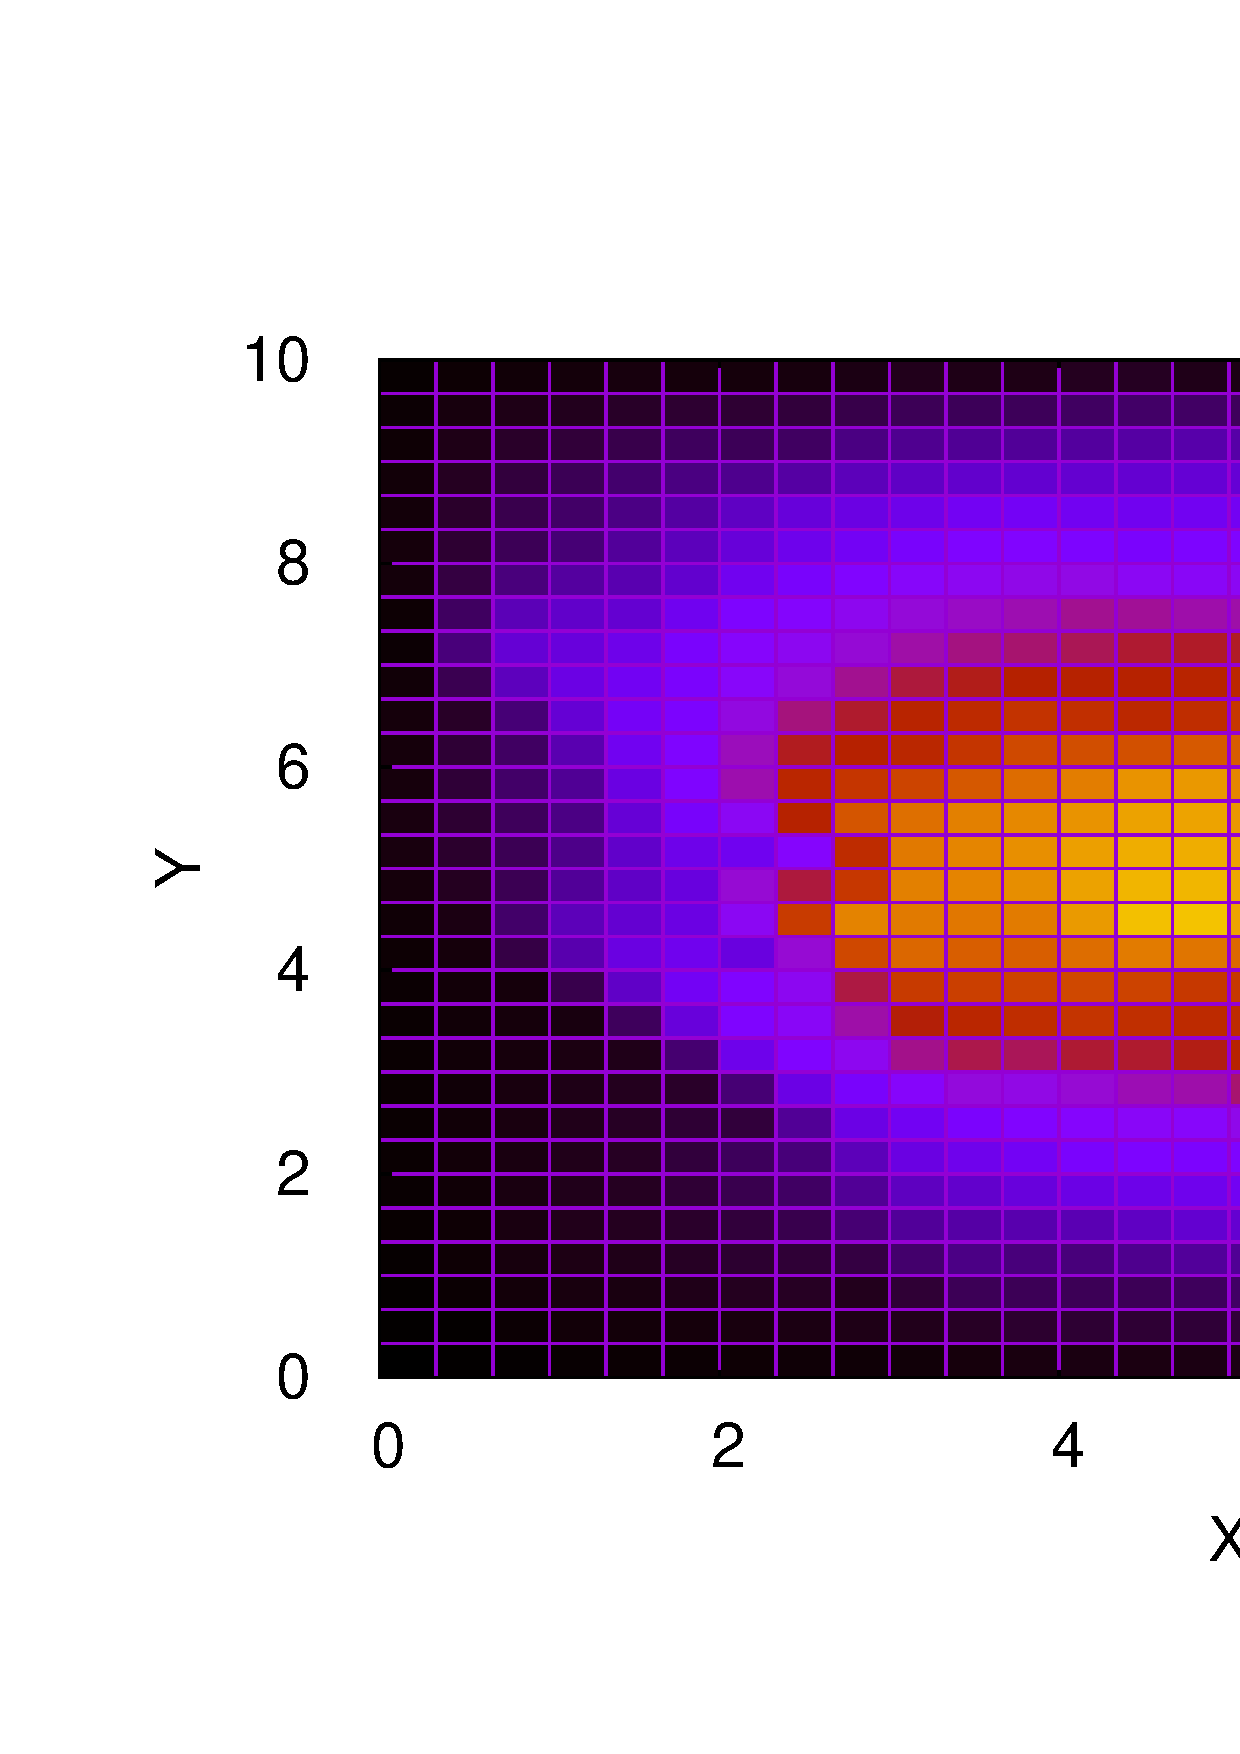
\includegraphics[width=\textwidth]{2DRandomDfig/45_map}
		\caption{the heat distribution map after 45 timesteps for the 2D heat problem}
		\label{fig:2d-randomD-45dt-map}
     \end{subfigure}
     \hfill     
        \caption{solving two-dimensional heat equation using CG method.}
        \label{fig:2d-CG-randomD}
\end{figure}

In contrast with the case of the constant diffusion coefficient, because of those random points which will not diffuse ($D(\vec{r}^{*})=0$), here the distribution of $\phi$ is not symmetric.

%stv
insert the plots for simple 2d and then the assignment here


\phantomsection
\section*{Appendix} % The \section*{} command stops section numbering
\addcontentsline{toc}{section}{Appendix} % Adds this section to the table of contents

As computer architecture advanced, it became more difficult to compare the performance of various computer systems simply by looking at their specifications. Therefore, tests were developed that allowed comparison of different architectures. For example, Pentium 4 processors generally operated at a higher clock frequency than Athlon XP or PowerPC processors, which did not necessarily translate to more computational power; a processor with a slower clock frequency might perform as well as or even better than a processor operating at a higher frequency \footnote{The megahertz myth, or less commonly the gigahertz myth, refers to the misconception of only using clock rate (for example measured in megahertz or gigahertz) to compare the performance of different microprocessors.}.
\\
Benchmarks are designed to mimic a particular type of workload on a component or system. Benchmarking is usually associated with assessing performance characteristics of computer hardware, for example, the floating point operation performance of a CPU.
\subsection*{PARKBENCH}
The PARKBENCH (PARallel Kernels and BENCHmarks) committee, originally called the Parallel Benchmark Working Group (PBWG) was founded at Supercomputing '92 in Minneapolis, when a group of about 50 people interested in computer benchmarking met under the joint initiative of Tony Hey and Jack Dongarra, and the chairmanship of Roger Hockney. The objectives of the PARKBENCH group are; 
\begin{itemize} 
\item To establish a comprehensive set of parallel benchmarks that is generally accepted by both users and vendors of parallel systems.

\item To provide a focus for parallel benchmark activities and avoid unnecessary duplication of effort and proliferation of benchmarks.
\item To set standards for benchmarking methodology and result-reporting together with a control database/repository for both the benchmarks and the results.
\item To make the benchmarks and results freely available in the public domain. 
\end{itemize}
	
Further information on PARKBENCH may be obtained at:\\
 \texttt{http://www.netlib.org/parkbench} .

\subsection*{NAS Parallel Benchmarks}

NAS Parallel Benchmarks (NPB) are a set of benchmarks targeting performance evaluation of highly parallel supercomputers. The NAS Parallel Benchmarks (NPB) are a small set of programs designed to help evaluate the performance of parallel supercomputers.  They are developed and maintained by the NASA Advanced Supercomputing (NAS) Division (formerly the NASA Numerical Aerodynamic Simulation Program) based at the NASA Ames Research Center.
The benchmarks are derived from computational fluid dynamics (CFD) applications and consist of five kernels and three pseudo-applications. The benchmark suite has been extended to include new benchmarks for unstructured adaptive meshes, parallel I/O, multi-zone applications, and computational grids. 
\\
The original eight benchmarks specified in NPB 1 mimic the computation and data movement in CFD applications:
\begin{itemize}
  \item IS - Integer Sort, random memory access
  \item EP - Embarrassingly Parallel
  \item CG - Conjugate Gradient, irregular memory access and communication
  \item MG - Multi-Grid on a sequence of meshes, long- and short-distance communication, memory intensive
  \item FT - discrete 3D fast Fourier Transform, all-to-all communication
  \item BT - Block Tri-diagonal solver
  \item SP - Scalar Penta-diagonal solver
  \item LU - Lower-Upper Gauss-Seidel solver
\end{itemize}
and there are several other benchmarks for unstructured computation, parallel I/O, and data movement.
\\
As of NPB 3.3, eleven benchmarks are defined. Further information on NAS may be obtained at: \\ \texttt{www.nas.nasa.gov/publications/npb.html} .
  
%\input{sections/sample}
%------------------------------------------------

  
\bibliographystyle{unsrt}
\bibliography{ref}

 
\end{document}